% Options for packages loaded elsewhere
\PassOptionsToPackage{unicode}{hyperref}
\PassOptionsToPackage{hyphens}{url}
%
\documentclass[
]{article}
\usepackage{amsmath,amssymb}
\usepackage{iftex}
\ifPDFTeX
  \usepackage[T1]{fontenc}
  \usepackage[utf8]{inputenc}
  \usepackage{textcomp} % provide euro and other symbols
\else % if luatex or xetex
  \usepackage{unicode-math} % this also loads fontspec
  \defaultfontfeatures{Scale=MatchLowercase}
  \defaultfontfeatures[\rmfamily]{Ligatures=TeX,Scale=1}
\fi
\usepackage{lmodern}
\ifPDFTeX\else
  % xetex/luatex font selection
\fi
% Use upquote if available, for straight quotes in verbatim environments
\IfFileExists{upquote.sty}{\usepackage{upquote}}{}
% microtype removed (compile time on Overleaf's free plan):
% \IfFileExists{microtype.sty}{% use microtype if available
%   \usepackage[]{microtype}
%   \UseMicrotypeSet[protrusion]{basicmath} % disable protrusion for tt fonts
% }{}
\makeatletter
\@ifundefined{KOMAClassName}{% if non-KOMA class
  \IfFileExists{parskip.sty}{%
    \usepackage{parskip}
  }{% else
    \setlength{\parindent}{0pt}
    \setlength{\parskip}{6pt plus 2pt minus 1pt}}
}{% if KOMA class
  \KOMAoptions{parskip=half}}
\makeatother
\usepackage{xcolor}
\usepackage[margin=2.5cm]{geometry}
\usepackage{longtable,booktabs,array}
\usepackage{calc} % for calculating minipage widths
% Correct order of tables after \paragraph or \subparagraph
\usepackage{etoolbox}
\makeatletter
\patchcmd\longtable{\par}{\if@noskipsec\mbox{}\fi\par}{}{}
\makeatother
% Allow footnotes in longtable head/foot
\IfFileExists{footnotehyper.sty}{\usepackage{footnotehyper}}{\usepackage{footnote}}
\makesavenoteenv{longtable}
\usepackage{graphicx}
\makeatletter
\def\maxwidth{\ifdim\Gin@nat@width>\linewidth\linewidth\else\Gin@nat@width\fi}
\def\maxheight{\ifdim\Gin@nat@height>\textheight\textheight\else\Gin@nat@height\fi}
\makeatother
% Scale images if necessary, so that they will not overflow the page
% margins by default, and it is still possible to overwrite the defaults
% using explicit options in \includegraphics[width, height, ...]{}
\setkeys{Gin}{width=\maxwidth,height=\maxheight,keepaspectratio}
% Set default figure placement to htbp
\makeatletter
\def\fps@figure{htbp}
\makeatother
\setlength{\emergencystretch}{3em} % prevent overfull lines
\providecommand{\tightlist}{%
  \setlength{\itemsep}{0pt}\setlength{\parskip}{0pt}}
\setcounter{secnumdepth}{-\maxdimen} % remove section numbering
\ifLuaTeX
  \usepackage{selnolig}  % disable illegal ligatures
\fi
\usepackage[]{natbib}
\bibliographystyle{plainnat}
\IfFileExists{bookmark.sty}{\usepackage{bookmark}}{\usepackage{hyperref}}
\IfFileExists{xurl.sty}{\usepackage{xurl}}{} % add URL line breaks if available
\urlstyle{same}
\hypersetup{
  pdftitle={Next-day rainfall forecasting for Sylhet, Bangladesh, from NASA POWER reanalysis data: a frozen-protocol comparison of baselines, classical machine learning and deep sequence models},
  hidelinks,
  pdfcreator={LaTeX via pandoc}}

\title{Next-day rainfall forecasting for Sylhet, Bangladesh, from NASA POWER reanalysis data: a frozen-protocol comparison of baselines, classical machine learning and deep sequence models}
\author{Mubarok Hossen Kamil\\
Department of Electrical and Electronic Engineering\\
Shahjalal University of Science and Technology (SUST), Sylhet 3114, Bangladesh}
\date{Draft manuscript, 17 October 2026}

\usepackage{amsmath,amssymb,booktabs,graphicx,hyperref,natbib}  % already loaded by the template; no-op, kept explicit
\usepackage{pdflscape}
\begin{document}
\maketitle

\hypertarget{abstract}{%
\section{Abstract}\label{abstract}}

Sylhet in north-eastern Bangladesh is among the wettest regions of the country, yet next-day rainfall guidance for a single location is rarely benchmarked against strong, honest reference forecasts. We compared five baselines, ten classical machine-learning models and three deep sequence models for next-day rain occurrence (at least 1 mm) and rainfall amount, using daily National Aeronautics and Space Administration (NASA) Prediction of Worldwide Energy Resources (POWER) data for one grid cell (1981--2025). All models used identical features and chronological splits, hyper-parameters were tuned on development years only, and the configuration was frozen before a single evaluation on the locked test years 2020--2025 (2,192 days).  % source: 09_derived_numbers.csv | * | test_days=2,192
On the test years, CatBoost reached a Brier skill score (BSS) of 0.376 {[}95 \% confidence interval (CI) 0.324, 0.423{]} against climatology, compared with 0.269 for a seasonal + persistence baseline.  % source: 07_test_cls_bootstrap.csv | index=catboost | BSS=0.376; BSS_lo=0.324; BSS_hi=0.423
 % source: 07_test_cls_bootstrap.csv | index=baseline:seasonal+persistence | BSS=0.269
All ten classical models and two of the three deep models improved on seasonal + persistence ($\Delta$BSS +0.070 to +0.108; Holm-adjusted Diebold--Mariano p $\le$ 0.0001), but none of these twelve differed significantly from the pre-declared LightGBM reference (smallest p\_Holm = 0.065).  % source: 09_derived_numbers.csv | * | famA_cls_learner_dBSS_min=0.070; famA_cls_learner_dBSS_max=0.108; famA_cls_learner_p_holm_max=0.0001
 % source: 09_derived_numbers.csv | * | famB_cls_learner_p_holm_min=0.065
For amounts, CatBoost with a Tweedie loss had the lowest mean absolute error (MAE, 8.534 mm versus 8.797 mm), but the difference was not significant after Holm correction (p\_Holm = 0.160).  % source: 07_test_reg_bootstrap.csv | index=catboost_tweedie | MAE=8.534
 % source: 07_test_reg_bootstrap.csv | index=baseline:seasonal+persistence | MAE=8.797
 % source: 07_statistical_comparison.csv | family=A & task=reg & loss=abs_error & model=catboost_tweedie | p_holm=0.160; significant=False
Only a seed ensemble of TSMixer significantly improved the mean squared error skill score (MSESS): $\Delta$MSESS +0.047, p\_Holm = 0.023.  % source: 07_statistical_comparison.csv | family=A & task=reg & loss=sq_error & model=deep:tsmixer | estimate=0.047; p_holm=0.023; significant=True
Skill came mainly from rain persistence; heavy rain was damped and lagged by one day, and the frozen forecasts showed almost no probabilistic skill against independent satellite rainfall from the Integrated Multi-satellitE Retrievals for the Global Precipitation Measurement mission (IMERG): CatBoost BSS 0.004.  % source: 07_imerg_secondary_cls.csv | index=catboost | vs IMERG/BSS=0.004
Machine learning added reliable but modest probabilistic skill over a strong baseline, whereas deep sequence models did not earn their computational cost at this single site.

\hypertarget{introduction}{%
\section{1 Introduction}\label{introduction}}

Bangladesh receives most of its rainfall during the summer monsoon, and the north-eastern Sylhet region is one of its wettest parts, with orographic enhancement along the hills that border the Meghalaya plateau \citep{shahid2010}. Floods, including flash floods in the haor wetlands of the Sylhet basin, strongly affect agriculture in this region \citep{brammer1990}. Short-range numerical weather prediction (NWP) is the usual basis of such forecasts, and statistical guidance derived from data has long complemented it \citep{wilks2019}. Here we ask whether data-driven models trained on local time series can provide useful next-day guidance at low cost.

Gridded reanalysis products make long, gap-free daily records available for any location. The NASA Prediction of Worldwide Energy Resources (POWER) service distributes daily meteorological variables derived mainly from the Modern-Era Retrospective analysis for Research and Applications, Version 2 (MERRA-2) \citep{gelaro2017, sparks2018}. MERRA-2 precipitation over land is corrected towards observation-based products \citep{reichle2017}, and POWER also offers satellite precipitation from the IMERG product of the Global Precipitation Measurement (GPM) mission \citep{huffman2020}, whose performance over Bangladesh has been evaluated by \citet{ahmed2021}. Such data are attractive for machine learning, but they also carry risks that are easy to overlook: inhomogeneities in the target series, inputs and target taken from the same model, and evaluation protocols that leak future information.

Gradient-boosted trees such as XGBoost \citep{chen2016xgboost}, LightGBM \citep{ke2017lightgbm} and CatBoost \citep{prokhorenkova2018} are strong learners for tabular data, and recent deep architectures for time series, including the Temporal Fusion Transformer (TFT) \citep{lim2021}, TSMixer \citep{chen2023tsmixer} and the Time-series Dense Encoder (TiDE) \citep{das2023tide}, are now easy to apply through libraries such as Darts \citep{herzen2022}. Forecast verification practice measures skill against reference forecasts such as climatology and persistence \citep{wilks2019}, and a fair comparison also requires chronological splits and an evaluation period that is not used for tuning. For a skewed, persistent variable such as daily rainfall, a forecast can look accurate while adding little to ``tomorrow is like today, adjusted for the season''.

This study therefore asked a deliberately narrow question: how much skill do classical and deep machine-learning models add to strong statistical baselines for next-day rainfall at one site in Sylhet, when every model uses identical inputs and splits and the test years are evaluated only once? The contributions are: (i) a leakage-tested, chronological benchmark of five baselines, ten classical models, several regression formulations and three deep sequence models for rain occurrence and amount; (ii) a final evaluation whose configuration was frozen before the test years were opened (an internal pre-registration, not a public registry) with paired block-bootstrap confidence intervals and Holm-corrected Diebold--Mariano (DM) tests \citep{diebold1995, harvey1997}; (iii) ablations of features, training window, rain-day threshold, look-back length and rainfall source; and (iv) an analysis of where the forecasts fail, including a check against independent satellite rainfall.

\hypertarget{study-area-and-data}{%
\section{2 Study area and data}\label{study-area-and-data}}

\hypertarget{study-area}{%
\subsection{2.1 Study area}\label{study-area}}

The study location was the NASA POWER grid point at 24.9157$^{\circ}$ N, 91.832$^{\circ}$ E in the Sylhet region of north-eastern Bangladesh. The elevation reported by POWER, 103.47 m, is the MERRA-2 mean elevation of the 0.5$^{\circ}$ $\times$ 0.625$^{\circ}$ grid cell, not the elevation of a station. Sylhet has a pronounced monsoon climate with most rain between June and September and a dry winter \citep{shahid2010}. We used four seasons: pre-monsoon (March--May), monsoon (June--September), post-monsoon (October--November) and winter (December--February).

\hypertarget{nasa-power-daily-data}{%
\subsection{2.2 NASA POWER daily data}\label{nasa-power-daily-data}}

Daily data for 1 January 1981 to 31 December 2025 were downloaded from the POWER Agroclimatology (AG) community on 14 October 2026 (file SHA-256 recorded in the repository). POWER defines days in Coordinated Universal Time (UTC); because Bangladesh time is UTC+6, one POWER day covers 06:00--06:00 local time. The variables are listed below. Most come from MERRA-2 \citep{gelaro2017}; shortwave radiation is labelled Clouds and the Earth's Radiant Energy System (CERES) SYN1deg in the file header, IMERG\_PRECTOT is satellite precipitation from IMERG \citep{huffman2020}. The header of our raw POWER file labels IMERG\_PRECTOT as ``MERRA-2 Total Precipitation (mm/day)'' despite its IMERG\_ prefix; we treated this as a labelling error because the series starts in 1998, when IMERG coverage begins in the file, and its annual totals differ clearly from those of PRECTOTCORR (Section 4.1). All variables are reanalysis or satellite estimates for a grid cell, not rain-gauge observations.

\begin{longtable}[]{@{}
  >{\raggedright\arraybackslash}p{(\columnwidth - 6\tabcolsep) * \real{0.3000}}
  >{\raggedright\arraybackslash}p{(\columnwidth - 6\tabcolsep) * \real{0.3600}}
  >{\raggedright\arraybackslash}p{(\columnwidth - 6\tabcolsep) * \real{0.1400}}
  >{\raggedright\arraybackslash}p{(\columnwidth - 6\tabcolsep) * \real{0.2000}}@{}}
\toprule\noalign{}
\begin{minipage}[b]{\linewidth}\raggedright
Variable
\end{minipage} & \begin{minipage}[b]{\linewidth}\raggedright
Description
\end{minipage} & \begin{minipage}[b]{\linewidth}\raggedright
Units
\end{minipage} & \begin{minipage}[b]{\linewidth}\raggedright
Use
\end{minipage} \\
\midrule\noalign{}
\endhead
\bottomrule\noalign{}
\endlastfoot
PRECTOTCORR & bias-corrected precipitation (MERRA-2) & mm/day & target and predictor \\
IMERG\_PRECTOT & satellite precipitation (IMERG, 1998--2025) & mm/day & secondary target only \\
T2M, T2M\_MAX, T2M\_MIN & 2 m air temperature: mean, maximum, minimum & $^{\circ}$C & predictors \\
T2MDEW & 2 m dew/frost point & $^{\circ}$C & predictor (Set B) \\
RH2M & 2 m relative humidity & \% & predictor \\
QV2M & 2 m specific humidity & g/kg & predictor (Set B) \\
PS & surface pressure & kPa & predictor (Set B) \\
WS2M, WS10M & wind speed at 2 m and 10 m & m/s & predictors (WS10M Set B) \\
WD2M & wind direction at 2 m & degrees & dropped (invalid from 31 Dec 2012) \\
ALLSKY\_SFC\_SW\_DWN & all-sky surface shortwave irradiance (1984--2025) & MJ/m$^{2}$/day & ablation only \\
\end{longtable}
\addtocounter{table}{-1}% uncaptioned table: no number

\hypertarget{data-audit-and-cleaning}{%
\subsection{2.3 Data audit and cleaning}\label{data-audit-and-cleaning}}

The raw file was never modified; a parsed copy only replaced the missing-value code $-$999 by missing values. Three problems were found and reported rather than silently corrected. First, every WD2M value from 31 December 2012 onwards was invalid (values between about $-$9,000 and $-$5,400), so WD2M was dropped. Second, IMERG\_PRECTOT starts in 1998 and radiation in 1984, so these variables were excluded from the main feature sets. Third, PRECTOTCORR is temporally inhomogeneous, with step changes around 2000 and 2016 that are not present in IMERG (Section 4.1); MERRA-2 land precipitation is corrected towards gauge-based observations, and changes over time in the underlying observing systems and gauge corrections can introduce temporal inhomogeneities \citep{reichle2017}; this is a plausible cause, but we did not test the attribution. A forward fill of interior gaps of at most two days was allowed, but no cell needed filling. The calendar columns YEAR and DOY were removed so that calendar year could not become a predictor of the 2016 regime.

\hypertarget{methods}{%
\section{3 Methods}\label{methods}}

\hypertarget{targets}{%
\subsection{3.1 Targets}\label{targets}}

The forecast for day t+1 was issued from information available at the end of day t. The primary classification target was rain on day t+1 of at least 1 mm (\texttt{y\_cls}), the standard wet-day definition of the Expert Team on Climate Change Detection and Indices (ETCCDI) \citep{zhang2011}; thresholds of 0.1 mm and 2.5 mm were sensitivity analyses. The regression target was the rainfall amount on day t+1 in mm (\texttt{y\_reg}). Log-target models were trained on log(1 + y) and back-transformed with the smearing estimator of \citet{duan1983}, \(\hat y = S \exp(\hat z) - 1\) with \(S\) the mean of the exponentiated log-scale residuals, estimated on an out-of-sample inner slice.

\hypertarget{features-and-leakage-tests}{%
\subsection{3.2 Features and leakage tests}\label{features-and-leakage-tests}}

Two feature sets were built from day-t information only. Feature Set A (71 features) used PRECTOTCORR, T2M, T2M\_MAX, T2M\_MIN, RH2M and WS2M; Feature Set B (115 features) added PS, QV2M, T2MDEW, WS10M and the dew-point depression (DPD).  % source: 09_derived_numbers.csv | * | n_features_A=71; n_features_B=115
Feature families were current values, lags of 1, 2, 3, 5 and 7 days (rain as log(1 + mm)), rolling means over 3, 7, 14 and 30 days, rolling log rain sums, wet/dry spell counters, one-day tendencies, the diurnal temperature range (DTR) and DPD, and day-of-year harmonics with the month; calendar year was never a feature. Rolling windows required complete windows, so the first 29 days were dropped, leaving 16,406 rows shared by both sets.  % source: 09_derived_numbers.csv | * | n_rows=16,406
Set B was used for all headline models; Set A was an ablation.

Leakage was tested automatically: (i) a truncation test recomputed the features after deleting all data after a random date and required identical feature values up to that date, with a deliberately leaky negative control that had to fail; (ii) the target had to equal the next calendar day's rainfall; (iii) no feature could equal the target; and (iv) a Spearman scan on training rows flagged any feature with \textbar $\rho$\textbar{} \textgreater{} 0.9 against the target. All tests passed; the largest correlation was 0.81, for today's rain.  % source: 02_leakage_correlation_scan_train.csv | index=rain_log1p | abs_max=0.81
 % source: 02_leakage_truncation_test.csv

\hypertarget{chronological-splits}{%
\subsection{3.3 Chronological splits}\label{chronological-splits}}

Rows were assigned to splits by the date of their target. Development used targets from 1981 to 2019, and the test period (targets 1 January 2020 to 31 December 2025) was locked behind a function that raised an error unless called with an explicit confirmation. Model selection used five expanding-window folds with training targets from 1981 up to 2004, 2007, 2010, 2013 or 2016 and validation on the following three years; a one-day purge removed the last training row so that no validation target was also the reference day of a training row (Fig. 2). Within each training fold, the last three target years formed an inner ``slice'' with the same purge; the slice was used to choose classification thresholds (maximum critical success index), early-stopping lengths and smearing factors, after which the model was refitted on the full training fold. The validation block was never used for any choice. Deep models used a single split (training targets 1981--2014, validation 2015--2019) because of their cost, with the 2012--2014 slice for early stopping. Scalers, imputers and encoders were fitted inside pipelines on training rows only. Random k-fold cross-validation was excluded; with random folds about 80 \% of validation targets appeared as same-day rain predictors of training rows.

Before the test years were touched, the complete configuration was frozen in \texttt{final\_config.yaml}: feature set, model list, hyper-parameters, seeds, per-seed thresholds, numbers of trees or epochs and smearing factors, all derived from an inner split of the development data (training targets up to 2016, slice 2017--2019). The final run refitted every model on all development targets up to 30 December 2019, predicted the 2,192 test days once, and wrote the predictions with a manifest of the code commit and configuration hash.  % source: 09_derived_numbers.csv | * | test_days=2,192
No model, threshold or test was changed afterwards.

\hypertarget{models}{%
\subsection{3.4 Models}\label{models}}

\textbf{Baselines.} Five baselines were fitted on training rows only: majority class / training mean; persistence (the empirical probability of rain given rain today, and ``tomorrow equals today'' for amounts); climatology (target day of year with a circular $\pm$7-day window); a seasonal model (logistic or ridge regression on two day-of-year harmonics); and seasonal + persistence, which adds today's rain flag or amount to the seasonal model. Seasonal + persistence was the main reference because exploratory analysis of the development years showed that season and persistence are the two sources of easy skill.

\textbf{Classical models.} For classification we used logistic regression without penalty and with L2, L1 and elastic-net penalties, logistic regression trained by stochastic gradient descent (SGD), random forest, XGBoost \citep{chen2016xgboost}, LightGBM \citep{ke2017lightgbm}, CatBoost \citep{prokhorenkova2018} and a multilayer perceptron (MLP); for regression the same families with linear, ridge, lasso, elastic-net and SGD regression and an MLP with Huber loss. Linear models used one-hot month encoding and standardisation inside a pipeline; classifiers used balanced class weights. Linear models, random forests and pipelines used scikit-learn \citep{pedregosa2011}. The MLP (two hidden layers) was implemented in PyTorch \citep{paszke2019} because the installed scikit-learn MLP did not support class weights, robust losses or a user-supplied chronological validation set.

\textbf{Regression formulations.} Four formulations were compared during development: direct squared-error regression in mm; regression of log(1 + mm) with naive and smeared back-transformation \citep{duan1983}; a two-stage hurdle model (probability of a wet day from the CatBoost classifier multiplied by a CatBoost amount model fitted on wet days with log target and smearing); and boosting with a Tweedie loss, whose compound Poisson--gamma case allows exact zeros and continuous positive amounts \citep{jorgensen1987}. CatBoost Tweedie and the hurdle model were carried to the final evaluation.

\textbf{Deep sequence models.} TSMixer \citep{chen2023tsmixer}, TiDE \citep{das2023tide} and TFT \citep{lim2021} were implemented with Darts 0.48.0 \citep{herzen2022}. Inputs were a 14-day look-back of the target and the nine other Set-B weather variables as past covariates, with day-of-year harmonics as known future covariates; the networks therefore learned their own temporal features. Rain occurrence was modelled with a Bernoulli likelihood; amounts were modelled in log space with smearing (TSMixer, TiDE) or with quantile regression at seven quantile levels from 0.05 to 0.95 (TFT, point forecast = mean of the quantile function). One-step forecasts were produced from observed look-backs. Each stochastic model was run with five seeds (0--4), and the seed-mean forecast was the tested forecast. We refer to all non-baseline models as learners.

\hypertarget{hyper-parameter-optimisation}{%
\subsection{3.5 Hyper-parameter optimisation}\label{hyper-parameter-optimisation}}

Classical models were tuned with Optuna \citep{akiba2019} using the tree-structured Parzen estimator (TPE) sampler (seed 42) and a median pruner applied to the running mean of the objective over the five folds. Objectives were BSS for classification and MAE for regression; the hurdle amount model was additionally tuned for the mean squared error skill score (MSESS). Budgets ranged from 15 trials (random forest) to 100 trials (SGD).  % source: 06_tuning_budget.csv | task=cls & model=random_forest | budget=15
 % source: 06_tuning_budget.csv | task=cls & model=sgd_logloss | budget=100
Because the best trial is selected on the same folds, the best parameters were re-run with seeds 1--4 to measure selection optimism. Deep models were tuned on the 2012--2014 slice only (20 trials for TSMixer and TiDE, 12 for TFT; one seed per trial) and then re-run with five seeds on the 2015--2019 validation years; the untuned default configuration was kept wherever tuning did not improve validation skill.

\hypertarget{verification-metrics}{%
\subsection{3.6 Verification metrics}\label{verification-metrics}}

Verification followed standard practice \citep{wilks2019}. Classification was scored with the Brier score and BSS, the area under the receiver operating characteristic (ROC) curve (ROC-AUC), the area under the precision--recall curve (PR-AUC), the expected calibration error (ECE, 10 equal-width bins), and, at the frozen threshold, the probability of detection (POD), false alarm ratio (FAR), critical success index (CSI) and Heidke skill score (HSS). With hits \(a\), false alarms \(b\), misses \(c\), correct negatives \(d\) and \(n = a+b+c+d\):

\[\mathrm{POD}=\frac{a}{a+c},\qquad \mathrm{FAR}=\frac{b}{a+b},\qquad \mathrm{CSI}=\frac{a}{a+b+c},\]

\[\mathrm{HSS}=\frac{2(ad-bc)}{(a+c)(c+d)+(a+b)(b+d)}.\]

For probabilities \(p_i\) and outcomes \(o_i\), \(\mathrm{BS}=\frac1n\sum_i (p_i-o_i)^2\) and \(\mathrm{BSS}=1-\mathrm{BS}/\mathrm{BS}_{\mathrm{ref}}\). Amounts were scored with MAE, root mean squared error (RMSE), bias, recall and precision for days of at least 20 and 50 mm, and \(\mathrm{MSESS}=1-\mathrm{MSE}/\mathrm{MSE}_{\mathrm{ref}}\). The reference for BSS and MSESS was climatology fitted on the same training rows; skill against seasonal + persistence was reported in addition because the climatology reference degraded when the target changed between decades (Section 4.3).

\hypertarget{statistical-testing}{%
\subsection{3.7 Statistical testing}\label{statistical-testing}}

Uncertainty was quantified with a paired block bootstrap \citep{kunsch1989} using calendar months of the target date as blocks (1,000 resamples, seed 42); the same blocks were used for all models so that differences are paired. Pairs of forecasts were compared with the DM test \citep{diebold1995} on daily loss differentials (squared error of probabilities, absolute error and squared error of amounts), using a Bartlett heteroskedasticity- and autocorrelation-consistent (HAC) variance \citep{newey1987} with bandwidth \(\lfloor 4(n/100)^{2/9}\rfloor\) (7 for the 2,192 test days), the small-sample correction of Harvey, Leybourne and Newbold (HLN) \citep{harvey1997} and a t distribution with n $-$ 1 degrees of freedom. Two families were pre-declared: family A compared every model with seasonal + persistence, and family B compared every model with the pre-declared headline reference (LightGBM for the Brier score, CatBoost Tweedie for absolute error, the hurdle model for squared error). p-values were adjusted with the Holm procedure \citep{holm1979} within each family, task and loss, at $\alpha$ = 0.05. Development-stage and ablation intervals are uncorrected bootstrap CIs and are described as such.

\hypertarget{ablations-error-analysis-and-interpretability}{%
\subsection{3.8 Ablations, error analysis and interpretability}\label{ablations-error-analysis-and-interpretability}}

Ablations changed one factor at a time on the development folds: feature set (A versus B; solar radiation from 1984), removal of each feature family, class weights, training window (from 1998, 2000 or 2010 onwards), rain-day threshold (0.1, 1 and 2.5 mm), look-back length of the deep models (14, 30 and 60 days) and rainfall source (IMERG instead of PRECTOTCORR as target and rain predictor, 1998--2019). Error analysis on the frozen test predictions was descriptive and stratified by month and season, observed intensity, year, local weather state of misses and false alarms, and dry-to-wet transitions. Interpretability used development data only: grouped permutation importance by feature family and physical variable, SHapley Additive exPlanations (SHAP) values from TreeExplainer \citep{lundberg2017}, accumulated local effects (ALE) \citep{apley2020} with partial dependence plots (PDP) for comparison, standardised linear coefficients across folds, and the variable-selection network (VSN) weights of TFT. The coverage of the TFT prediction intervals on the test years (Section 4.5) was computed in the final reporting stage from the frozen test predictions; like the error analysis, it was descriptive and changed no model, threshold or test.

\hypertarget{results}{%
\section{4 Results}\label{results}}

\hypertarget{data-audit-and-baselines}{%
\subsection{4.1 Data audit and baselines}\label{data-audit-and-baselines}}

The PRECTOTCORR series contained two step changes. Mean annual totals were 1,925 mm in 1981--1997, 2,970 mm in 1998--2015 and 5,377 mm in 2016--2025, whereas IMERG was nearly constant (3,680 mm and 3,757 mm for 1998--2015 and 2016--2025; Fig. 1).  % source: 09_derived_numbers.csv | * | prectotcorr_mean_1981_1997=1,925; prectotcorr_mean_1998_2015=2,970; prectotcorr_mean_2016_2025=5,377
 % source: 09_derived_numbers.csv | * | imerg_mean_1998_2015=3,680; imerg_mean_2016_2025=3,757
Pettitt tests \citep{pettitt1979} located change points with first years 2000 (p = 0.0000007, PRECTOTCORR 1981--2025) and 2015 (p = 0.0002, 1998--2025), but none for IMERG (p = 1.0); the PRECTOTCORR/IMERG ratio rose from 0.82 to 1.44.  % source: 01_pettitt_tests.csv | index=PRECTOTCORR 1981-2025 | p_value=0.0000007
 % source: 01_pettitt_tests.csv | index=PRECTOTCORR 1998-2025 | p_value=0.0002
 % source: 01_pettitt_tests.csv | index=IMERG_PRECTOT 1998-2025 | p_value=1.0
 % source: 01_pettitt_tests.csv | index=ratio 1998-2025 | mean_before=0.82; mean_after=1.44
The share of wet days (at least 1 mm) was 49.4 \% in the development years and 55.7 \% in the test years, whose mean rainfall was 14.13 mm/day with a maximum of 202 mm.  % source: 02_threshold_evidence.csv | index=>= 1.0 mm | rain_day_share=49.4%
 % source: 09_derived_numbers.csv | * | test_wet_share=55.7%; test_mean_mm=14.13; test_max_mm=202
The 1-mm threshold gave the highest agreement with IMERG on the same day (Cohen's $\kappa$ = 0.750).  % source: 02_threshold_evidence.csv | index=>= 1.0 mm | kappa_IMERG=0.750

Daily rain was persistent (lag-1 autocorrelation 0.58), so persistence and season set a high bar.  % source: 01_acf_pacf_lags1-7.csv | lag=1 | ACF_PRECTOTCORR=0.58
In the development folds, seasonal + persistence reached BSS 0.184 $\pm$ 0.058 (mean $\pm$ SD over folds), MAE 7.079 mm and MSESS 0.228, while persistence alone had a negative BSS ($-$0.020) and climatology had a ROC-AUC of 0.928.  % source: 03_baseline_cv_summary_y_cls.csv | index=seasonal+persistence | BSS/mean=0.184; BSS/std=0.058
 % source: 03_baseline_cv_summary_y_reg.csv | index=seasonal+persistence | MAE/mean=7.079; MSESS/mean=0.228
 % source: 03_baseline_cv_summary_y_cls.csv | index=persistence | BSS/mean=-0.020
 % source: 03_baseline_cv_summary_y_cls.csv | index=climatology | ROC_AUC/mean=0.928

\hypertarget{development-cross-validation-target-formulations-and-tuning}{%
\subsection{4.2 Development cross-validation, target formulations and tuning}\label{development-cross-validation-target-formulations-and-tuning}}

Tuning improved the gradient-boosted classifiers by small but consistent amounts: tuned LightGBM, CatBoost and XGBoost reached cross-validated BSS of 0.265, 0.265 and 0.263, gains of 0.006, 0.004 and 0.005 over their defaults that were positive in every fold.  % source: 06_default_vs_tuned.csv | task=cls & model=lightgbm | tuned=0.265; $\Delta$=0.006
 % source: 06_default_vs_tuned.csv | task=cls & model=catboost | tuned=0.265; $\Delta$=0.004
 % source: 06_default_vs_tuned.csv | task=cls & model=xgboost | tuned=0.263; $\Delta$=0.005
These gains were of the same size as the selection optimism of the best trial, 0.003--0.004 BSS when the best parameters were re-run with seeds 1--4.  % source: 09_derived_numbers.csv | * | seed0_optimism_lightgbm=0.003; seed0_optimism_catboost=0.004
Tuning repaired the unconverged SGD classifier (BSS 0.189 to 0.253) but left the penalised logistic models practically unchanged (L1: +0.0007).  % source: 06_default_vs_tuned.csv | task=cls & model=sgd_logloss | default=0.189; tuned=0.253
 % source: 06_default_vs_tuned.csv | task=cls & model=logreg_l1 | $\Delta$=0.0007

For amounts, the ranking depended on the loss. Naive back-transformation of log forecasts under-predicted strongly (CatBoost bias $-$4.774 mm/day), and Duan smearing reduced the bias to $-$1.071 mm/day with a smearing factor of 1.587.  % source: 04_jensen_log_backtransform.csv | index=catboost | bias/log_naive=-4.774; bias/log_smear=-1.071; smear_factor=1.587
The tuned CatBoost Tweedie model had the lowest cross-validated MAE (6.897 mm versus 7.079 mm for seasonal + persistence), whereas the hurdle model reached the highest MSESS; its MSESS was insensitive to the tuning objective (0.276 default, 0.278 MAE-tuned, 0.275 MSESS-tuned).  % source: 06_default_vs_tuned.csv | task=reg & model=catboost_tweedie | tuned=6.897
 % source: 03_baseline_cv_summary_y_reg.csv | index=seasonal+persistence | MAE/mean=7.079
 % source: 06_hurdle_mae_vs_msess.csv | model=hurdle_catboost_log | MSESS=0.276
 % source: 06_hurdle_mae_vs_msess.csv | model=hurdle_catboost_log_tuned | MSESS=0.278
 % source: 06_hurdle_mae_vs_msess.csv | model=hurdle_catboost_log_msess_tuned | MSESS=0.275
Ridge regression was re-tuned on a wider range because its first optimum lay on the upper boundary; the new optimum ($\alpha$ = 236) was interior.  % source: 09_derived_numbers.csv | * | ridge_alpha_retuned=236

Deep-model tuning on the 2012--2014 slice did not transfer to the 2015--2019 validation years. TFT classification changed from BSS 0.307 (default) to 0.305 (tuned), and TSMixer regression MAE worsened from 9.19 mm to 9.59 mm; only the TiDE classifier, whose default had not converged within the epoch budget, improved (0.186 to 0.214; $\Delta$BSS +0.027, bootstrap CI 0.016--0.040).  % source: 06_deep_cost_vs_skill.csv | model=tft default & task=cls | value=0.307
 % source: 06_deep_cost_vs_skill.csv | model=tft tuned & task=cls | value=0.305
 % source: 06_deep_cost_vs_skill.csv | model=tsmixer default & task=reg | value=9.19
 % source: 06_deep_cost_vs_skill.csv | model=tsmixer tuned & task=reg | value=9.59
 % source: 06_deep_cost_vs_skill.csv | model=tide default & task=cls | value=0.186
 % source: 06_deep_cost_vs_skill.csv | model=tide tuned & task=cls | value=0.214
 % source: 06_deep_tuned_vs_default_bootstrap.csv | model=tide & task=cls | estimate=0.027; ci_low=0.016; ci_high=0.040
The frozen deep configurations were therefore the defaults, except for the TiDE classifier.

\hypertarget{test-set-classification}{%
\subsection{4.3 Test-set classification}\label{test-set-classification}}

Table 1 lists all models on the test years. All learners except TiDE beat every baseline. CatBoost had the highest BSS (0.376 {[}0.324, 0.423{]}), followed closely by TFT (0.372), XGBoost (0.369) and LightGBM (0.368); the five logistic models reached 0.351--0.360, the MLP 0.357, TSMixer 0.342 and random forest 0.338.  % source: 07_test_cls_bootstrap.csv | index=catboost | BSS=0.376; BSS_lo=0.324; BSS_hi=0.423
 % source: 07_test_cls_bootstrap.csv | index=deep:tft | BSS=0.372
 % source: 07_test_cls_bootstrap.csv | index=xgboost | BSS=0.369
 % source: 07_test_cls_bootstrap.csv | index=lightgbm | BSS=0.368
 % source: 07_test_cls_bootstrap.csv | index=logreg_l1 | BSS=0.351
 % source: 07_test_cls_bootstrap.csv | index=sgd_logloss | BSS=0.360
 % source: 07_test_cls_bootstrap.csv | index=mlp | BSS=0.357
 % source: 07_test_cls_bootstrap.csv | index=deep:tsmixer | BSS=0.342
 % source: 07_test_cls_bootstrap.csv | index=random_forest | BSS=0.338
Discrimination was uniformly high (ROC-AUC 0.968--0.972 for the classical models), so the models differed mainly in calibration and sharpness; the boosters had the lowest ECE (0.018--0.023).  % source: 07_test_cls_bootstrap.csv | index=random_forest | ROC_AUC=0.968
 % source: 07_test_cls_bootstrap.csv | index=catboost | ROC_AUC=0.972; ECE=0.023
 % source: 07_test_cls_bootstrap.csv | index=xgboost | ECE=0.018

Against seasonal + persistence (BSS 0.269 {[}0.213, 0.321{]}), the improvements of all 12 learners other than TiDE (the ten classical models, TFT and TSMixer) ranged from $\Delta$BSS +0.070 to +0.108 and were all significant after Holm correction (largest p\_Holm 0.0001; Table 2, Fig. 3).  % source: 07_test_cls_bootstrap.csv | index=baseline:seasonal+persistence | BSS=0.269; BSS_lo=0.213; BSS_hi=0.321
 % source: 09_derived_numbers.csv | * | famA_cls_learner_dBSS_min=0.070; famA_cls_learner_dBSS_max=0.108; famA_cls_learner_p_holm_max=0.0001; famA_cls_learners_significant=12
TiDE was significantly worse than the baseline ($\Delta$BSS $-$0.042 {[}$-$0.066, $-$0.017{]}, p\_Holm = 0.008).  % source: 07_statistical_comparison.csv | family=A & task=cls & model=deep:tide | estimate=-0.042; ci_low=-0.066; ci_high=-0.017; p_holm=0.008; significant=True
No model was significantly better or worse than the pre-declared LightGBM reference except TiDE and the baselines: CatBoost differed by +0.008 {[}$-$0.002, 0.018{]} (p\_Holm = 1.000) and TFT by +0.004 {[}$-$0.017, 0.025{]} (p\_Holm = 1.000).  % source: 07_statistical_comparison.csv | family=B & task=cls & model=catboost | estimate=0.008; ci_low=-0.002; ci_high=0.018; p_holm=1.000; significant=False
 % source: 07_statistical_comparison.csv | family=B & task=cls & model=deep:tft | estimate=0.004; ci_low=-0.017; ci_high=0.025; p_holm=1.000; significant=False
Random forest was the only learner whose bootstrap CI against LightGBM excluded zero ($-$0.030 {[}$-$0.051, $-$0.009{]}), but this difference was not significant after Holm correction (p\_Holm = 0.065).  % source: 07_statistical_comparison.csv | family=B & task=cls & model=random_forest | estimate=-0.030; ci_low=-0.051; ci_high=-0.009; p_holm=0.065; significant=False

Test-set BSS values against climatology were higher than in development for every model (by +0.093 to +0.117 for the classical learners and +0.085 for seasonal + persistence).  % source: 09_derived_numbers.csv | * | test_minus_dev_BSS_learner_min=0.093; test_minus_dev_BSS_learner_max=0.117
 % source: 07_dev_vs_test_ranking.csv | task=cls & metric=BSS & model=baseline:seasonal+persistence | test - dev=0.085
We traced this to the reference rather than to leakage: climatology fitted mostly on the drier pre-2016 years is a poorer forecast in the wetter test years, so skill against seasonal + persistence (Table 1) is the more conservative headline. The ranking of models was stable between development and test (Spearman $\rho$ = 0.89 for BSS).  % source: 09_derived_numbers.csv | * | spearman_dev_test_BSS=0.89

\begin{landscape}
\footnotesize\setlength{\tabcolsep}{2pt}
\begin{tabular}{llrllllllll}
\toprule
Model & Family & Seeds & BSS [95\% CI] & BSS seed SD & BSS\_vs\_seas\_pers & ROC\_AUC & PR\_AUC & CSI & HSS & ECE \\
\midrule
Majority / mean & baseline & 1 & -1.529 [-2.134, -1.106] & 0.000 & -2.457 & 0.500 & 0.557 & 0.000 & 0.000 & 0.062 \\
Persistence & baseline & 1 & 0.130 [0.011, 0.228] & 0.000 & -0.189 & 0.908 & 0.888 & 0.848 & 0.815 & 0.057 \\
Climatology & baseline & 1 & 0.000 [0.000, 0.000] & 0.000 & -0.367 & 0.937 & 0.945 & 0.808 & 0.764 & 0.063 \\
Seasonal & baseline & 1 & -0.011 [-0.023, 0.002] & 0.000 & -0.383 & 0.937 & 0.947 & 0.807 & 0.764 & 0.065 \\
Seasonal + persistence & baseline & 1 & 0.269 [0.213, 0.321] & 0.000 & 0.000 & 0.960 & 0.964 & 0.858 & 0.826 & 0.053 \\
Logistic regression & classical & 1 & 0.360 [0.293, 0.416] & 0.000 & 0.124 & 0.969 & 0.975 & 0.862 & 0.827 & 0.018 \\
Logistic L2 (ridge) & classical & 1 & 0.358 [0.300, 0.408] & 0.000 & 0.123 & 0.970 & 0.975 & 0.867 & 0.836 & 0.030 \\
Logistic L1 (lasso) & classical & 5 & 0.351 [0.293, 0.402] & 0.000 & 0.112 & 0.970 & 0.976 & 0.867 & 0.838 & 0.037 \\
Logistic elastic net & classical & 5 & 0.358 [0.299, 0.408] & 0.000 & 0.122 & 0.970 & 0.975 & 0.868 & 0.837 & 0.029 \\
SGD (log loss) & classical & 5 & 0.360 [0.299, 0.409] & 0.000 & 0.124 & 0.970 & 0.975 & 0.866 & 0.833 & 0.028 \\
Random forest & classical & 5 & 0.338 [0.290, 0.380] & 0.001 & 0.096 & 0.968 & 0.972 & 0.855 & 0.813 & 0.038 \\
XGBoost & classical & 5 & 0.369 [0.314, 0.414] & 0.006 & 0.137 & 0.971 & 0.976 & 0.857 & 0.818 & 0.018 \\
LightGBM & classical & 5 & 0.368 [0.314, 0.414] & 0.003 & 0.136 & 0.971 & 0.976 & 0.860 & 0.823 & 0.020 \\
CatBoost & classical & 5 & 0.376 [0.324, 0.423] & 0.005 & 0.147 & 0.972 & 0.977 & 0.863 & 0.825 & 0.023 \\
MLP & classical & 5 & 0.357 [0.296, 0.407] & 0.003 & 0.121 & 0.969 & 0.974 & 0.860 & 0.824 & 0.022 \\
TSMixer & deep & 5 & 0.342 [0.282, 0.390] & 0.010 & 0.100 & 0.971 & 0.977 & 0.864 & 0.832 & 0.042 \\
TiDE & deep & 5 & 0.227 [0.164, 0.284] & 0.004 & -0.057 & 0.947 & 0.944 & 0.845 & 0.801 & 0.037 \\
TFT & deep & 5 & 0.372 [0.317, 0.420] & 0.018 & 0.141 & 0.972 & 0.977 & 0.873 & 0.842 & 0.034 \\
\bottomrule
\end{tabular}

\normalsize
\end{landscape}

\begin{landscape}
\footnotesize\setlength{\tabcolsep}{2pt}
\begin{tabular}{llrllllllll}
\toprule
Model & Family & Seeds & MAE [95\% CI] & MAE seed SD & MSESS [95\% CI] & MSESS\_vs\_seas\_pers & RMSE & bias & recall\_ge50 & precision\_ge50 \\
\midrule
Majority / mean & baseline & 1 & 14.300 [12.031, 16.631] & 0.000 & -0.227 [-0.282, -0.184] & -0.947 & 25.674 & -6.462 & 0.000 & -- \\
Persistence & baseline & 1 & 9.596 [7.588, 11.585] & 0.000 & 0.249 [0.082, 0.379] & -0.192 & 20.086 & 0.000 & 0.497 & 0.497 \\
Climatology & baseline & 1 & 10.696 [8.270, 13.113] & 0.000 & 0.000 [0.000, 0.000] & -0.587 & 23.180 & -6.480 & 0.000 & -- \\
Seasonal & baseline & 1 & 10.784 [8.382, 13.168] & 0.000 & -0.003 [-0.009, 0.004] & -0.591 & 23.210 & -6.444 & 0.000 & -- \\
Seasonal + persistence & baseline & 1 & 8.797 [7.010, 10.586] & 0.000 & 0.370 [0.307, 0.420] & 0.000 & 18.401 & -3.323 & 0.210 & 0.714 \\
Linear regression & classical & 1 & 9.369 [7.481, 11.276] & 0.000 & 0.320 [0.292, 0.347] & -0.080 & 19.120 & -2.336 & 0.012 & 0.667 \\
Ridge & classical & 1 & 9.300 [7.377, 11.205] & 0.000 & 0.306 [0.278, 0.333] & -0.102 & 19.316 & -2.752 & 0.012 & 0.667 \\
Lasso & classical & 1 & 9.224 [7.246, 11.187] & 0.000 & 0.275 [0.249, 0.304] & -0.150 & 19.731 & -3.505 & 0.006 & 1.000 \\
Elastic net & classical & 1 & 9.261 [7.259, 11.237] & 0.000 & 0.265 [0.239, 0.293] & -0.167 & 19.875 & -3.614 & 0.006 & 1.000 \\
SGD regressor & classical & 5 & 9.236 [7.331, 11.139] & 0.060 & 0.305 [0.276, 0.335] & -0.103 & 19.323 & -2.900 & 0.012 & 1.000 \\
Random forest & classical & 5 & 8.734 [6.916, 10.593] & 0.004 & 0.374 [0.319, 0.418] & 0.007 & 18.340 & -2.428 & 0.192 & 0.582 \\
XGBoost & classical & 5 & 8.864 [6.999, 10.707] & 0.023 & 0.388 [0.314, 0.442] & 0.028 & 18.138 & -1.799 & 0.269 & 0.625 \\
LightGBM & classical & 5 & 8.774 [6.940, 10.615] & 0.019 & 0.395 [0.329, 0.446] & 0.041 & 18.024 & -1.889 & 0.269 & 0.592 \\
CatBoost & classical & 5 & 8.799 [6.961, 10.629] & 0.020 & 0.387 [0.326, 0.432] & 0.028 & 18.144 & -2.132 & 0.228 & 0.644 \\
MLP (Huber) & classical & 5 & 8.744 [6.820, 10.676] & 0.095 & 0.343 [0.305, 0.374] & -0.043 & 18.792 & -4.521 & 0.126 & 0.724 \\
CatBoost Tweedie & classical & 5 & 8.534 [6.711, 10.359] & 0.037 & 0.395 [0.334, 0.439] & 0.039 & 18.035 & -2.739 & 0.222 & 0.661 \\
Hurdle CatBoost (log + smearing) & classical & 5 & 9.534 [7.588, 11.497] & 0.063 & 0.396 [0.291, 0.474] & 0.042 & 18.009 & 1.663 & 0.491 & 0.529 \\
TSMixer & deep & 5 & 9.299 [7.579, 11.009] & 1.919 & 0.417 [0.356, 0.468] & 0.075 & 17.694 & -0.070 & 0.305 & 0.637 \\
TiDE & deep & 5 & 9.687 [7.710, 11.605] & 0.048 & 0.370 [0.286, 0.436] & -0.001 & 18.406 & 0.602 & 0.455 & 0.547 \\
TFT & deep & 5 & 8.604 [6.789, 10.446] & 0.190 & 0.373 [0.322, 0.415] & 0.005 & 18.358 & -2.908 & 0.060 & 0.769 \\
\bottomrule
\end{tabular}

\normalsize
\end{landscape}

\hypertarget{test-set-regression}{%
\subsection{4.4 Test-set regression}\label{test-set-regression}}

Table 3 lists the amount forecasts. CatBoost Tweedie had the lowest MAE (8.534 mm {[}6.711, 10.359{]}) against 8.797 mm for seasonal + persistence; the paired difference was $-$0.263 mm {[}$-$0.493, $-$0.031{]}, with a raw DM p = 0.023 that did not survive Holm correction (p\_Holm = 0.160).  % source: 07_test_reg_bootstrap.csv | index=catboost_tweedie | MAE=8.534; MAE_lo=6.711; MAE_hi=10.359
 % source: 07_test_reg_bootstrap.csv | index=baseline:seasonal+persistence | MAE=8.797
 % source: 07_statistical_comparison.csv | family=A & task=reg & loss=abs_error & model=catboost_tweedie | estimate=-0.263; ci_low=-0.493; ci_high=-0.031; p=0.023; p_holm=0.160; significant=False
No model was significantly better than seasonal + persistence in MAE, and seven were significantly worse: the four penalised and unpenalised linear models other than lasso, the hurdle model, TSMixer and TiDE (Table 4); lasso narrowly missed significance (p\_Holm = 0.053).  % source: 09_derived_numbers.csv | * | famA_mae_better_significant=0; famA_mae_worse_significant=7
 % source: 07_statistical_comparison.csv | family=A & task=reg & loss=abs_error & model=lasso | p_holm=0.053; significant=False

The squared-error view ranked the models differently. TSMixer had the highest MSESS (0.417 {[}0.356, 0.468{]}), ahead of the hurdle model (0.396), CatBoost Tweedie (0.395) and LightGBM (0.395), against 0.370 for seasonal + persistence.  % source: 07_test_reg_bootstrap.csv | index=deep:tsmixer | MSESS=0.417; MSESS_lo=0.356; MSESS_hi=0.468
 % source: 07_test_reg_bootstrap.csv | index=hurdle_catboost_log_msess | MSESS=0.396
 % source: 07_test_reg_bootstrap.csv | index=catboost_tweedie | MSESS=0.395
 % source: 07_test_reg_bootstrap.csv | index=lightgbm | MSESS=0.395
 % source: 07_test_reg_bootstrap.csv | index=baseline:seasonal+persistence | MSESS=0.370
The TSMixer seed ensemble was the only model significantly better than seasonal + persistence on squared error ($\Delta$MSESS +0.047 {[}0.019, 0.076{]}, p\_Holm = 0.023), while lasso and elastic net were significantly worse (p\_Holm = 0.030 and 0.020).  % source: 07_statistical_comparison.csv | family=A & task=reg & loss=sq_error & model=deep:tsmixer | estimate=0.047; ci_low=0.019; ci_high=0.076; p_holm=0.023; significant=True
 % source: 07_statistical_comparison.csv | family=A & task=reg & loss=sq_error & model=lasso | p_holm=0.030; significant=True
 % source: 07_statistical_comparison.csv | family=A & task=reg & loss=sq_error & model=elasticnet | p_holm=0.020; significant=True
The two views reflect the target formulation: median-type forecasts (Tweedie loss) minimise absolute error but under-estimate amounts (bias $-$2.74 mm/day), whereas mean-type forecasts (hurdle with smearing) are nearly unbiased or slightly high (+1.66 mm/day) and detect more heavy-rain days (recall for days $\ge$ 50 mm 0.49 versus 0.22 for Tweedie and 0.21 for seasonal + persistence).  % source: 07_test_reg_bootstrap.csv | index=catboost_tweedie | bias=-2.74; recall_ge50=0.22
 % source: 07_test_reg_bootstrap.csv | index=hurdle_catboost_log_msess | bias=1.66; recall_ge50=0.49
 % source: 07_test_reg_bootstrap.csv | index=baseline:seasonal+persistence | recall_ge50=0.21

Seed variation mattered for one deep model. TSMixer seed 1, whose early stopping on the slice had already stopped at epoch 1 during the freeze, produced a test MAE of 13.2 mm; the seed-mean forecast was robust (9.299 mm) but the per-seed SD of MAE was 1.919 mm.  % source: 07_test_reg_per_seed.csv | model=deep:tsmixer & seed=1 | MAE=13.2
 % source: 07_test_reg_bootstrap.csv | index=deep:tsmixer | MAE=9.299
 % source: 09_paper_table3.csv | Model=TSMixer | MAE seed SD=1.919

As a secondary check, the frozen forecasts were scored against IMERG rainfall on the same test days. Discrimination was largely retained (CatBoost ROC-AUC 0.921), but probabilistic skill vanished (CatBoost BSS 0.004; range $-$0.074 to 0.029 across all learners), and MSESS against IMERG ranged from $-$0.115 (hurdle) to 0.179 (TFT).  % source: 07_imerg_secondary_cls.csv | index=catboost | vs IMERG/ROC_AUC=0.921; vs IMERG/BSS=0.004
 % source: 07_imerg_secondary_cls.csv | index=deep:tide | vs IMERG/BSS=-0.074
 % source: 07_imerg_secondary_cls.csv | index=deep:tft | vs IMERG/BSS=0.029
 % source: 07_imerg_secondary_reg.csv | index=hurdle_catboost_log_msess | vs IMERG/MSESS=-0.115
 % source: 07_imerg_secondary_reg.csv | index=deep:tft | vs IMERG/MSESS=0.179

\begin{landscape}
\footnotesize\setlength{\tabcolsep}{2pt}
\begin{longtable}{lrllllllll}
\caption{Test-set regression of rainfall (mm) on day t+1, 2020-2025. Point estimates of the seed-mean forecast with 95 \% monthly block-bootstrap CIs; 'MAE seed SD' is the standard deviation of the per-seed MAE. MSESS is relative to climatology and 'MSESS vs s+p' to seasonal + persistence (s+p); bias in mm/day; recall and precision for days of at least 50 mm.} \label{tab:3} \\
\toprule
Model & Seeds & MAE [95\% CI] & MAE seed SD & MSESS [95\% CI] & MSESS vs s+p & RMSE & Bias & Recall $\ge$50 mm & Precision $\ge$50 mm \\
\midrule
\endfirsthead
\caption[]{Test-set regression of rainfall (mm) on day t+1, 2020-2025. Point estimates of the seed-mean forecast with 95 \% monthly block-bootstrap CIs; 'MAE seed SD' is the standard deviation of the per-seed MAE. MSESS is relative to climatology and 'MSESS vs s+p' to seasonal + persistence (s+p); bias in mm/day; recall and precision for days of at least 50 mm.} \\
\toprule
Model & Seeds & MAE [95\% CI] & MAE seed SD & MSESS [95\% CI] & MSESS vs s+p & RMSE & Bias & Recall $\ge$50 mm & Precision $\ge$50 mm \\
\midrule
\endhead
\midrule
\multicolumn{10}{r}{Continued on next page} \\
\midrule
\endfoot
\bottomrule
\endlastfoot
Majority / mean & 1 & 14.300 [12.031, 16.631] & 0.000 & -0.227 [-0.282, -0.184] & -0.947 & 25.674 & -6.462 & 0.000 & -- \\
Persistence & 1 & 9.596 [7.588, 11.585] & 0.000 & 0.249 [0.082, 0.379] & -0.192 & 20.086 & 0.000 & 0.497 & 0.497 \\
Climatology & 1 & 10.696 [8.270, 13.113] & 0.000 & 0.000 [0.000, 0.000] & -0.587 & 23.180 & -6.480 & 0.000 & -- \\
Seasonal & 1 & 10.784 [8.382, 13.168] & 0.000 & -0.003 [-0.009, 0.004] & -0.591 & 23.210 & -6.444 & 0.000 & -- \\
Seasonal + persistence & 1 & 8.797 [7.010, 10.586] & 0.000 & 0.370 [0.307, 0.420] & 0.000 & 18.401 & -3.323 & 0.210 & 0.714 \\
Linear regression & 1 & 9.369 [7.481, 11.276] & 0.000 & 0.320 [0.292, 0.347] & -0.080 & 19.120 & -2.336 & 0.012 & 0.667 \\
Ridge & 1 & 9.300 [7.377, 11.205] & 0.000 & 0.306 [0.278, 0.333] & -0.102 & 19.316 & -2.752 & 0.012 & 0.667 \\
Lasso & 1 & 9.224 [7.246, 11.187] & 0.000 & 0.275 [0.249, 0.304] & -0.150 & 19.731 & -3.505 & 0.006 & 1.000 \\
Elastic net & 1 & 9.261 [7.259, 11.237] & 0.000 & 0.265 [0.239, 0.293] & -0.167 & 19.875 & -3.614 & 0.006 & 1.000 \\
SGD regressor & 5 & 9.236 [7.331, 11.139] & 0.060 & 0.305 [0.276, 0.335] & -0.103 & 19.323 & -2.900 & 0.012 & 1.000 \\
Random forest & 5 & 8.734 [6.916, 10.593] & 0.004 & 0.374 [0.319, 0.418] & 0.007 & 18.340 & -2.428 & 0.192 & 0.582 \\
XGBoost & 5 & 8.864 [6.999, 10.707] & 0.023 & 0.388 [0.314, 0.442] & 0.028 & 18.138 & -1.799 & 0.269 & 0.625 \\
LightGBM & 5 & 8.774 [6.940, 10.615] & 0.019 & 0.395 [0.329, 0.446] & 0.041 & 18.024 & -1.889 & 0.269 & 0.592 \\
CatBoost & 5 & 8.799 [6.961, 10.629] & 0.020 & 0.387 [0.326, 0.432] & 0.028 & 18.144 & -2.132 & 0.228 & 0.644 \\
MLP (Huber) & 5 & 8.744 [6.820, 10.676] & 0.095 & 0.343 [0.305, 0.374] & -0.043 & 18.792 & -4.521 & 0.126 & 0.724 \\
CatBoost Tweedie & 5 & 8.534 [6.711, 10.359] & 0.037 & 0.395 [0.334, 0.439] & 0.039 & 18.035 & -2.739 & 0.222 & 0.661 \\
Hurdle CatBoost (log + smearing) & 5 & 9.534 [7.588, 11.497] & 0.063 & 0.396 [0.291, 0.474] & 0.042 & 18.009 & 1.663 & 0.491 & 0.529 \\
TSMixer & 5 & 9.299 [7.579, 11.009] & 1.919 & 0.417 [0.356, 0.468] & 0.075 & 17.694 & -0.070 & 0.305 & 0.637 \\
TiDE & 5 & 9.687 [7.710, 11.605] & 0.048 & 0.370 [0.286, 0.436] & -0.001 & 18.406 & 0.602 & 0.455 & 0.547 \\
TFT & 5 & 8.604 [6.789, 10.446] & 0.190 & 0.373 [0.322, 0.415] & 0.005 & 18.358 & -2.908 & 0.060 & 0.769 \\
\end{longtable}

\normalsize
\end{landscape}

\begin{landscape}
\footnotesize\setlength{\tabcolsep}{2pt}
\begin{longtable}{lllllll}
\caption{Paired test-set comparisons for regression: $\Delta$MAE (mm; negative = better) and $\Delta$MSESS (positive = better) with 95 \% block-bootstrap CIs and Holm-adjusted Diebold-Mariano p-values (p\_Holm, by metric and family; * significant at 0.05). Family A: versus seasonal + persistence (s+p); family B: versus CatBoost Tweedie.} \label{tab:4} \\
\toprule
Model & $\Delta$MAE vs s+p & p\_Holm (MAE, A) & $\Delta$MSESS vs s+p & p\_Holm (MSESS, A) & $\Delta$MAE vs Tweedie & p\_Holm (MAE, B) \\
\midrule
\endfirsthead
\caption[]{Paired test-set comparisons for regression: $\Delta$MAE (mm; negative = better) and $\Delta$MSESS (positive = better) with 95 \% block-bootstrap CIs and Holm-adjusted Diebold-Mariano p-values (p\_Holm, by metric and family; * significant at 0.05). Family A: versus seasonal + persistence (s+p); family B: versus CatBoost Tweedie.} \\
\toprule
Model & $\Delta$MAE vs s+p & p\_Holm (MAE, A) & $\Delta$MSESS vs s+p & p\_Holm (MSESS, A) & $\Delta$MAE vs Tweedie & p\_Holm (MAE, B) \\
\midrule
\endhead
\midrule
\multicolumn{7}{r}{Continued on next page} \\
\midrule
\endfoot
\bottomrule
\endlastfoot
Majority / mean & +5.504 [+4.638, +6.412] & <0.001* & -0.597 [-0.677, -0.513] & <0.001* & +5.767 [+4.960, +6.632] & <0.001* \\
Persistence & +0.799 [+0.392, +1.204] & <0.001* & -0.121 [-0.226, -0.037] & 0.003* & +1.062 [+0.569, +1.528] & <0.001* \\
Climatology & +1.899 [+1.248, +2.583] & <0.001* & -0.370 [-0.420, -0.307] & <0.001* & +2.162 [+1.530, +2.792] & <0.001* \\
Seasonal & +1.987 [+1.323, +2.661] & <0.001* & -0.372 [-0.427, -0.306] & <0.001* & +2.250 [+1.602, +2.878] & <0.001* \\
Seasonal + persistence & ref. & ref. & ref. & ref. & +0.263 [+0.031, +0.493] & 0.068 \\
Linear regression & +0.572 [+0.282, +0.884] & 0.001* & -0.050 [-0.090, +0.004] & 0.405 & +0.835 [+0.592, +1.090] & <0.001* \\
Ridge & +0.503 [+0.192, +0.825] & 0.006* & -0.064 [-0.106, -0.010] & 0.152 & +0.766 [+0.506, +1.035] & <0.001* \\
Lasso & +0.427 [+0.062, +0.794] & 0.053 & -0.094 [-0.139, -0.033] & 0.030* & +0.690 [+0.377, +1.033] & <0.001* \\
Elastic net & +0.464 [+0.082, +0.854] & 0.041* & -0.105 [-0.151, -0.041] & 0.020* & +0.727 [+0.399, +1.081] & <0.001* \\
SGD regressor & +0.439 [+0.130, +0.757] & 0.024* & -0.065 [-0.105, -0.011] & 0.152 & +0.702 [+0.428, +0.996] & <0.001* \\
Random forest & -0.063 [-0.245, +0.123] & 1.000 & +0.004 [-0.029, +0.037] & 1.000 & +0.200 [+0.063, +0.338] & 0.014* \\
XGBoost & +0.067 [-0.179, +0.295] & 1.000 & +0.018 [-0.022, +0.068] & 1.000 & +0.330 [+0.199, +0.476] & <0.001* \\
LightGBM & -0.023 [-0.286, +0.234] & 1.000 & +0.026 [-0.015, +0.082] & 1.000 & +0.240 [+0.112, +0.370] & <0.001* \\
CatBoost & +0.002 [-0.228, +0.219] & 1.000 & +0.017 [-0.020, +0.065] & 1.000 & +0.265 [+0.166, +0.357] & <0.001* \\
MLP (Huber) & -0.052 [-0.332, +0.266] & 1.000 & -0.027 [-0.068, +0.020] & 1.000 & +0.211 [-0.017, +0.471] & 0.068 \\
CatBoost Tweedie & -0.263 [-0.493, -0.031] & 0.160 & +0.025 [-0.010, +0.068] & 1.000 & ref. & ref. \\
Hurdle CatBoost (log + smearing) & +0.737 [+0.232, +1.206] & 0.001* & +0.027 [-0.047, +0.086] & 1.000 & +1.001 [+0.504, +1.507] & <0.001* \\
TSMixer & +0.502 [+0.239, +0.745] & 0.002* & +0.047 [+0.019, +0.076] & 0.023* & +0.765 [+0.543, +0.984] & <0.001* \\
TiDE & +0.891 [+0.577, +1.207] & <0.001* & -0.000 [-0.034, +0.026] & 1.000 & +1.154 [+0.816, +1.461] & <0.001* \\
TFT & -0.193 [-0.400, +0.011] & 0.333 & +0.003 [-0.032, +0.045] & 1.000 & +0.070 [-0.050, +0.194] & 0.326 \\
\end{longtable}

\normalsize
\end{landscape}

\hypertarget{deep-versus-classical-models}{%
\subsection{4.5 Deep versus classical models}\label{deep-versus-classical-models}}

On the identical deep-learning split (validation 2015--2019), tuned LightGBM reached BSS 0.329 with about 9 s per fit, whereas TFT reached 0.307 at 228 s per fit (default) and 0.305 at 651 s (tuned); seasonal + persistence reached 0.224.  % source: 06_deep_cost_vs_skill.csv | model=lightgbm_tuned & task=cls | value=0.329; fit_s=9
 % source: 06_deep_cost_vs_skill.csv | model=tft default & task=cls | value=0.307; fit_s=228
 % source: 06_deep_cost_vs_skill.csv | model=tft tuned & task=cls | value=0.305; fit_s=651
 % source: 06_deep_cost_vs_skill.csv | model=seasonal+persistence & task=cls | value=0.224
On the test years, TFT was not significantly different from LightGBM ($\Delta$BSS +0.004, p\_Holm = 1.000), TSMixer was slightly but not significantly worse ($-$0.027 {[}$-$0.054, 0.003{]}, p\_Holm = 0.447), and TiDE was significantly worse ($-$0.142, p\_Holm \textless{} 0.001).  % source: 07_statistical_comparison.csv | family=B & task=cls & model=deep:tft | estimate=0.004; p_holm=1.000; significant=False
 % source: 07_statistical_comparison.csv | family=B & task=cls & model=deep:tsmixer | estimate=-0.027; ci_low=-0.054; ci_high=0.003; p_holm=0.447; significant=False
 % source: 07_statistical_comparison.csv | family=B & task=cls & model=deep:tide | estimate=-0.142; significant=True

The deep models nevertheless had distinctive regression behaviour. TiDE and TSMixer, trained in log space with smearing, produced mean-type forecasts with small bias (+0.602 and $-$0.070 mm/day) and higher heavy-rain recall (0.455 and 0.305) than the boosters, at the cost of significantly larger absolute errors (p\_Holm \textless{} 0.001 and = 0.002).  % source: 07_test_reg_bootstrap.csv | index=deep:tide | bias=0.602; recall_ge50=0.455
 % source: 07_test_reg_bootstrap.csv | index=deep:tsmixer | bias=-0.070; recall_ge50=0.305
 % source: 07_statistical_comparison.csv | family=A & task=reg & loss=abs_error & model=deep:tide | significant=True
 % source: 07_statistical_comparison.csv | family=A & task=reg & loss=abs_error & model=deep:tsmixer | p_holm=0.002; significant=True
TFT is a probabilistic model; its 80 \% and 90 \% central intervals covered 85.2 \% and 92.5 \% of the test days (seed mean), compared with 82.1 \% and 89.2 \% in the 2015--2019 validation years, so the intervals were slightly conservative on the test years (SD across seeds 1.3 percentage points for the 80 \% interval), and 6.1 \% of test days exceeded the 0.95 quantile.  % source: 09_tft_interval_coverage_test.csv | quantity=coverage80 | mean=85.2%; std=1.3%
 % source: 09_tft_interval_coverage_test.csv | quantity=coverage90 | mean=92.5%
 % source: 09_tft_interval_coverage_test.csv | quantity=share_above_q95 | mean=6.1%
 % source: 05_deep_regression_L14.csv | model=tft & target=qmean | coverage80=82.1%; coverage90=89.2%
Its quantile-mean point forecast had a test MAE of 8.604 mm, but the forecast was strongly damped for heavy rain (recall for days $\ge$ 50 mm 0.060).  % source: 07_test_reg_bootstrap.csv | index=deep:tft | MAE=8.604; recall_ge50=0.060

\hypertarget{ablations}{%
\subsection{4.6 Ablations}\label{ablations}}

Shorter training windows hurt every model, even though the excluded early years belong to a different PRECTOTCORR regime. Training only on 2010 onwards (folds 4--5) reduced the BSS of LightGBM by 0.061 {[}0.028, 0.091{]} and of L1-logistic regression by 0.060, and increased the MAE of CatBoost Tweedie by 0.481 mm and of the hurdle model by 0.514 mm (uncorrected bootstrap CIs).  % source: 06_ablation_master.csv | variant=win_2010 & model=lightgbm & metric=dBSS | estimate=abs(0.061); ci_low=abs(0.091); ci_high=abs(0.028)
 % source: 06_ablation_master.csv | variant=win_2010 & model=logreg_l1 & metric=dBSS | estimate=abs(0.060)
 % source: 06_ablation_master.csv | variant=win_2010 & model=catboost_tweedie & metric=dMAE | estimate=0.481
 % source: 06_ablation_master.csv | variant=win_2010 & model=hurdle_catboost_log_msess & metric=dMAE | estimate=0.514
Training from 2000 also hurt L1-logistic regression ($\Delta$BSS $-$0.027) and CatBoost Tweedie ($\Delta$MAE +0.220 mm).  % source: 06_ablation_master.csv | variant=win_2000 & model=logreg_l1 & metric=dBSS | estimate=-0.027
 % source: 06_ablation_master.csv | variant=win_2000 & model=catboost_tweedie & metric=dMAE | estimate=0.220

Feature choices mattered little. Set A performed like Set B (LightGBM $\Delta$BSS $-$0.002 {[}$-$0.009, 0.004{]}), solar radiation added nothing ($-$0.002), and removing any single feature family changed the boosters' BSS by less than 0.005 in absolute value; only L1-logistic regression lost skill without the season family ($-$0.014 {[}$-$0.020, $-$0.007{]}, uncorrected bootstrap CI).  % source: 06_ablation_master.csv | variant=set_A & model=lightgbm & metric=dBSS | estimate=-0.002; ci_low=-0.009; ci_high=0.004
 % source: 06_ablation_master.csv | variant=B+solar_1984 & model=lightgbm & metric=dBSS | estimate=-0.002
 % source: 06_ablation_master.csv | variant=drop_tendency & model=lightgbm & metric=dBSS | estimate=abs(0.005)
 % source: 06_ablation_master.csv | variant=drop_season & model=logreg_l1 & metric=dBSS | estimate=-0.014; ci_low=-0.020; ci_high=-0.007
The advantage of LightGBM over L1-logistic regression was +0.019 {[}0.004, 0.035{]} at 0.1 mm but +0.011 {[}$-$0.003, 0.027{]} at 1 mm and +0.006 at 2.5 mm, so the ranking was stable across thresholds while the gap was clear only at the lowest one.  % source: 06_ablation_master.csv | variant=thr 0.1 folds all & model=lightgbm & metric=dBSS | estimate=0.019; ci_low=0.004; ci_high=0.035
 % source: 06_ablation_master.csv | variant=thr 1.0 folds all & model=lightgbm & metric=dBSS | estimate=0.011; ci_low=-0.003; ci_high=0.027
 % source: 06_ablation_master.csv | variant=thr 2.5 folds all & model=lightgbm & metric=dBSS | estimate=0.006

With IMERG as target and rain predictor, LightGBM reached a cross-validated BSS of only 0.159, compared with 0.259 for PRECTOTCORR over the same years, yet the booster--logistic ranking was preserved (+0.011 {[}$-$0.002, 0.025{]}).  % source: 06_ablation_summary.csv | task=cls & model=lightgbm & variant=imerg_1998 | BSS=0.159
 % source: 06_ablation_summary.csv | task=cls & model=lightgbm & variant=win_1998 | BSS=0.259
 % source: 06_ablation_master.csv | variant=IMERG folds all & model=lightgbm & metric=dBSS | estimate=0.011; ci_low=-0.002; ci_high=0.025
For the deep models, a look-back of 14 days was never beaten: 30 days increased the MAE of TSMixer (mm target) by 0.370 mm and of TFT by 0.167 mm.  % source: 06_ablation_master.csv | variant=tsmixer mm L30 & model=tsmixer & metric=dMAE | estimate=0.370
 % source: 06_ablation_master.csv | variant=tft mm L30 & model=tft & metric=dMAE | estimate=0.167
Of 118 ablation contrasts, 68 were classified as noise, 20 as model-specific and 30 as solid, without multiplicity correction (Fig. 7).  % source: 09_derived_numbers.csv | * | ablation_contrasts=118; ablation_noise=68; ablation_model-specific=20; ablation_solid=30

\hypertarget{where-the-forecasts-succeed-and-fail}{%
\subsection{4.7 Where the forecasts succeed and fail}\label{where-the-forecasts-succeed-and-fail}}

Skill varied strongly with season. In the transition months (March, April, October and November) the learners reached monthly BSS of 0.41--0.49, but in the core monsoon (June--September) only 0.09--0.34, because almost every monsoon day is wet and the remaining uncertainty is in the few dry days (Fig. 8).  % source: 09_derived_numbers.csv | * | transition_month_bss_min=0.41; transition_month_bss_max=0.49; monsoon_month_bss_min=0.09; monsoon_month_bss_max=0.34
In the test monsoon, LightGBM reached BSS 0.219 against 0.106 for seasonal + persistence.  % source: 07_test_by_season_cls.csv | season=monsoon & model=lightgbm | BSS=0.219
 % source: 07_test_by_season_cls.csv | season=monsoon & model=baseline:seasonal+persistence | BSS=0.106
Calibration was good in every season; LightGBM's monsoon ECE was 0.009, while seasonal + persistence under-forecast monsoon rain (mean probability 0.906 versus an observed frequency of 0.958).  % source: 08_calibration_by_season.csv | season=monsoon & model=lightgbm | ECE=0.009
 % source: 08_calibration_by_season.csv | season=monsoon & model=baseline:seasonal+persistence | mean_forecast=0.906; observed_frequency=0.958

Heavy rain was systematically damped. On the 167 test days with at least 50 mm (mean 83.3 mm), the learners' mean forecasts were only 32--62 \% of the observed amount (CatBoost Tweedie 37.0 mm, hurdle 51.6 mm; Fig. 9).  % source: 08_errors_by_intensity.csv | task=reg & bin=$\ge$ 50 mm & model=catboost_tweedie | n_days=167; obs_mean=83.3; fc_mean=37.0
 % source: 08_errors_by_intensity.csv | task=reg & bin=$\ge$ 50 mm & model=hurdle_catboost_log_msess | fc_mean=51.6
 % source: 09_derived_numbers.csv | * | heavy_ratio_min=32%; heavy_ratio_max=62%
The forecasts were also lagged: on the day after a heavy-rain day the Tweedie forecast was higher (45.1 mm) than on the heavy day itself, and its correlation with the previous day's observation (0.873) exceeded that with the target day (0.712).  % source: 09_derived_numbers.csv | * | tweedie_heavy_fc_nextday=45.1; tweedie_corr_previous_day=0.873; tweedie_corr_target_day=0.712
Rain onsets after a dry day were caught in 41--59 \% of cases by the learners, compared with 35 \% for seasonal + persistence, whereas cessations after a wet day were rarely forecast (14--24 \%).  % source: 09_derived_numbers.csv | * | onset_caught_min=41%; onset_caught_max=59%; cessation_caught_min=14%; cessation_caught_max=24%
 % source: 08_transitions.csv | subset=dry today (onset?) & model=baseline:seasonal+persistence | transitions_caught=35%
Missed rain days (LightGBM) typically followed a dry day with low humidity (median rain today 0.05 mm, RH2M 73.6 \%) and brought light rain (median 2.78 mm).  % source: 08_fn_fp_states.csv | outcome=FN | rain_today_mm=0.05; RH2M=73.6; rain_tomorrow_mm=2.78

Interpretation on the development folds showed that recent rain dominated. The rain-memory group accounted for 42.4 \% of LightGBM's mean absolute SHAP value and 55.4 \% of its grouped permutation importance (66.4 \% for CatBoost Tweedie), followed by temperature (20.1 \% of SHAP) and moisture (17.3 \%); pressure, season and wind contributed less (Fig. 10).  % source: 08_importance_consolidated.csv | index=rain memory | LightGBM SHAP share (%)=42.4; LightGBM perm. $\Delta$Brier share (%)=55.4; Tweedie perm. $\Delta$MAE share (%)=66.4
 % source: 08_importance_consolidated.csv | index=temperature | LightGBM SHAP share (%)=20.1
 % source: 08_importance_consolidated.csv | index=moisture | LightGBM SHAP share (%)=17.3
The TFT variable-selection weights ranked season (40.9 \%) and moisture (38.2 \%) first, because TFT receives rain history as its target sequence rather than through the selection network.  % source: 08_importance_consolidated.csv | index=season | TFT VSN weight (%)=40.9
 % source: 08_importance_consolidated.csv | index=moisture | TFT VSN weight (%)=38.2

\hypertarget{discussion}{%
\section{5 Discussion}\label{discussion}}

The central result is that machine learning added a modest but reliable amount of probabilistic skill to a strong statistical baseline. The gain in BSS over seasonal + persistence of about 0.07--0.11 was significant for every classical model and for TFT and TSMixer (Holm-adjusted p $\le$ 0.0001), whereas the differences among the good models were an order of magnitude smaller and not significant (Table 2).  % source: 09_derived_numbers.csv | * | famA_cls_learner_p_holm_max=0.0001
This pattern, where the choice between learners matters far less than the choice of a good reference, is a direct consequence of the data: next-day rainfall at one grid cell is dominated by persistence and season, and both are available to every model. Regularised logistic regression captured most of the gain, so a simple, interpretable model is a defensible operational choice when probability forecasts are the goal.

For amounts, no model beat seasonal + persistence significantly in MAE (the best, CatBoost Tweedie, had p\_Holm = 0.160), and the ranking depended on the error measure.  % source: 07_statistical_comparison.csv | family=A & task=reg & loss=abs_error & model=catboost_tweedie | p_holm=0.160; significant=False
Median-type forecasts (Tweedie loss) minimised absolute error but under-estimated amounts, while mean-type forecasts (hurdle with Duan smearing, TiDE and TSMixer in log space) were nearly unbiased and detected more heavy-rain days but had larger absolute errors. Reporting MAE, MSESS and bias together is therefore necessary; any single metric would have produced a misleading winner. The smearing correction was essential for log-target models \citep{duan1983}.

Deep sequence models did not earn their computational cost here. TFT was not significantly different from the boosters for probabilities but cost more than an order of magnitude more training time and offered reasonably calibrated quantiles, TiDE was the weakest learner for occurrence, and TSMixer showed that a single unlucky seed can fail. With about 14,000 development days at one location, the data volume is small for networks with hundreds of thousands of parameters, the tabular models already receive hand-crafted temporal features, and in our experiments deep-model tuning on 2012--2014 did not transfer to 2015--2019 (Section 4.2).

The most important caveat is the target. PRECTOTCORR is a corrected reanalysis product with documented inhomogeneities \citep{reichle2017}, and the step change around 2016 made the test years wetter than the development years. Skill measured against climatology was inflated by this change, which is why we report skill against seasonal + persistence as the headline. More fundamentally, the frozen forecasts retained discrimination but lost almost all probabilistic skill when scored against IMERG. Because predictors and target come from the same reanalysis system, part of the measured skill may reflect internal consistency of MERRA-2 rather than predictability of observed rainfall. Studies that use POWER rainfall for machine learning should therefore validate against independent rainfall, ideally rain-gauge records of the Bangladesh Meteorological Department (BMD), and IMERG evaluations for Bangladesh \citep{ahmed2021} suggest that satellite products are themselves imperfect references.

The error analysis explains where the skill comes from. The models were most useful in the transition seasons, when rain is neither certain nor rare, and least useful in the core monsoon. Heavy rain was damped and lagged by a day, the signature of an adjusted-persistence forecast without information about approaching weather systems. Organised precipitation systems in and around Bangladesh, including pre-monsoon convective storms (nor'westers) and monsoon systems \citep{rafiuddin2010}, develop or arrive from outside the grid cell and cannot be anticipated from local surface variables alone; upstream fields or NWP output would be needed.

\hypertarget{limitations-and-future-work}{%
\section{6 Limitations and future work}\label{limitations-and-future-work}}

\begin{enumerate}
\def\labelenumi{\arabic{enumi}.}
\tightlist
\item
  \textbf{Reanalysis target.} The target is MERRA-2 PRECTOTCORR for a 0.5$^{\circ}$ $\times$ 0.625$^{\circ}$ grid cell, not rain-gauge data, and predictors and target come from the same system; skill against IMERG was close to zero. Future work should evaluate against BMD gauges in Sylhet and against IMERG as a primary target.  % source: 08_limitations_summary.csv
\item
  \textbf{Single grid cell.} All 115 predictors are local; no spatial or upstream information was used. Multi-cell or gridded inputs and convolutional or graph models are natural extensions.
\item
  \textbf{Inhomogeneous target.} PRECTOTCORR has step changes around 2000 and 2016; we documented but did not correct them. Homogenisation or training on IMERG would test robustness.
\item
  \textbf{Seasonal imbalance.} Almost all monsoon days are wet, so within-monsoon discrimination rests on few dry days (31 in the test monsoon seasons).
\item
  \textbf{Heavy rain.} Extremes were under-predicted and lagged; quantile or extreme-value losses and NWP inputs are needed for warning applications.
\item
  \textbf{Sample size for deep models.} 14,214 development days are small relative to the 412,927 parameters of the tuned TFT classifier; deep-model tuning did not transfer between periods.  % source: 09_derived_numbers.csv | * | n_dev_rows=14,214; tft_cls_tuned_parameters=412,927
\item
  \textbf{Hindcast, not an operational system.} No NWP inputs were used, and the forecasts were not compared with operational NWP or BMD forecasts, which are the relevant baselines for practical use; POWER days are UTC rather than a local gauge reporting day; and POWER data are published with a latency of weeks, so day-t inputs are not available in real time.
\item
  \textbf{Non-stationarity.} Test errors were larger and skill against climatology higher than in development; shorter recent windows did not help.
\item
  \textbf{Single test period and multiplicity.} One six-year test window was evaluated; development-stage contrasts and the 118 ablation contrasts were not corrected for multiplicity, and tuned cross-validation scores carry selection optimism.
\item
  \textbf{Interpretability.} Collinear predictors limit attributions to groups of variables; importance does not imply causation.
\end{enumerate}

\hypertarget{conclusion}{%
\section{7 Conclusion}\label{conclusion}}

Using a leakage-tested, chronological protocol frozen before testing, we found that gradient-boosted trees, regularised logistic regression and TFT all provided significantly better next-day rain probabilities for Sylhet than a seasonal + persistence baseline (Holm-adjusted p $\le$ 0.0001), with no significant differences among them,  % source: 09_derived_numbers.csv | * | famA_cls_learner_p_holm_max=0.0001
while no model significantly improved the absolute error of amount forecasts. Deep sequence models did not justify their cost, and the skill largely disappeared against independent satellite rainfall. Honest baselines, frozen configurations and independent verification data are therefore at least as important as the choice of algorithm for data-driven rainfall forecasting from reanalysis data.

\hypertarget{reproducibility-and-data-availability}{%
\section{8 Reproducibility and data availability}\label{reproducibility-and-data-availability}}

All code, notebooks, tables and figures are in the project repository at https://github.com/mhkamil/sylhet-rainfall-forecasting. The raw POWER file is stored read-only with its SHA-256 hash; processed data are regenerated by the numbered notebooks, each of which reads from \texttt{data/processed} and writes its outputs to disk. Package versions are pinned in \texttt{requirements.txt} (Python 3.13, pandas 3.0.5, scikit-learn 1.9.1, XGBoost 3.4.1, LightGBM 4.7.0, CatBoost 1.2.10, PyTorch 2.14.1, Darts 0.48.0, Optuna 5.0.0, SHAP 0.54.1). The frozen configuration is \texttt{final\_config.yaml} (pre-test commit \texttt{827eae8}); the one-shot test predictions are in \texttt{models/test/} together with \texttt{manifest.json}, which records the commit (\texttt{55d416f}) and the configuration hash. The protocol is enforced by 118 unit tests, which pass on the final code: 107 for the forecasting pipeline (leakage, splits, metrics, runner, MLP, deep models, tuning, ablations and the freeze) and 11 for the manuscript checker and LaTeX export. Every number in the Abstract and Results is linked by a source comment to a CSV table in \texttt{reports/tables/}, and \texttt{notebooks/09\_paper\_tables.ipynb} re-checks all of them, regenerates Tables 1--4 and converts this manuscript to pdfLaTeX-ready LaTeX with pandoc 3.1.3, packages an Overleaf bundle (\texttt{reports/overleaf\_bundle.zip}) and compiles it to \texttt{reports/paper\_draft.pdf}. Seeds were fixed throughout (stochastic models: seeds 0--4; Optuna sampler and bootstrap: seed 42). Data: NASA Langley Research Center (LaRC) Prediction Of Worldwide Energy Resources (POWER) Project, Agroclimatology (AG) daily point data for 24.9157$^{\circ}$ N, 91.832$^{\circ}$ E, 1981--2025, downloaded on 14 October 2026 from https://power.larc.nasa.gov/ (download date as recorded in \texttt{data/raw/DATA\_SOURCE.md}) \citep{sparks2018, gelaro2017, reichle2017, huffman2020}.

\hypertarget{figures-and-tables}{%
\section{Figures and tables}\label{figures-and-tables}}

\begin{figure}
\centering
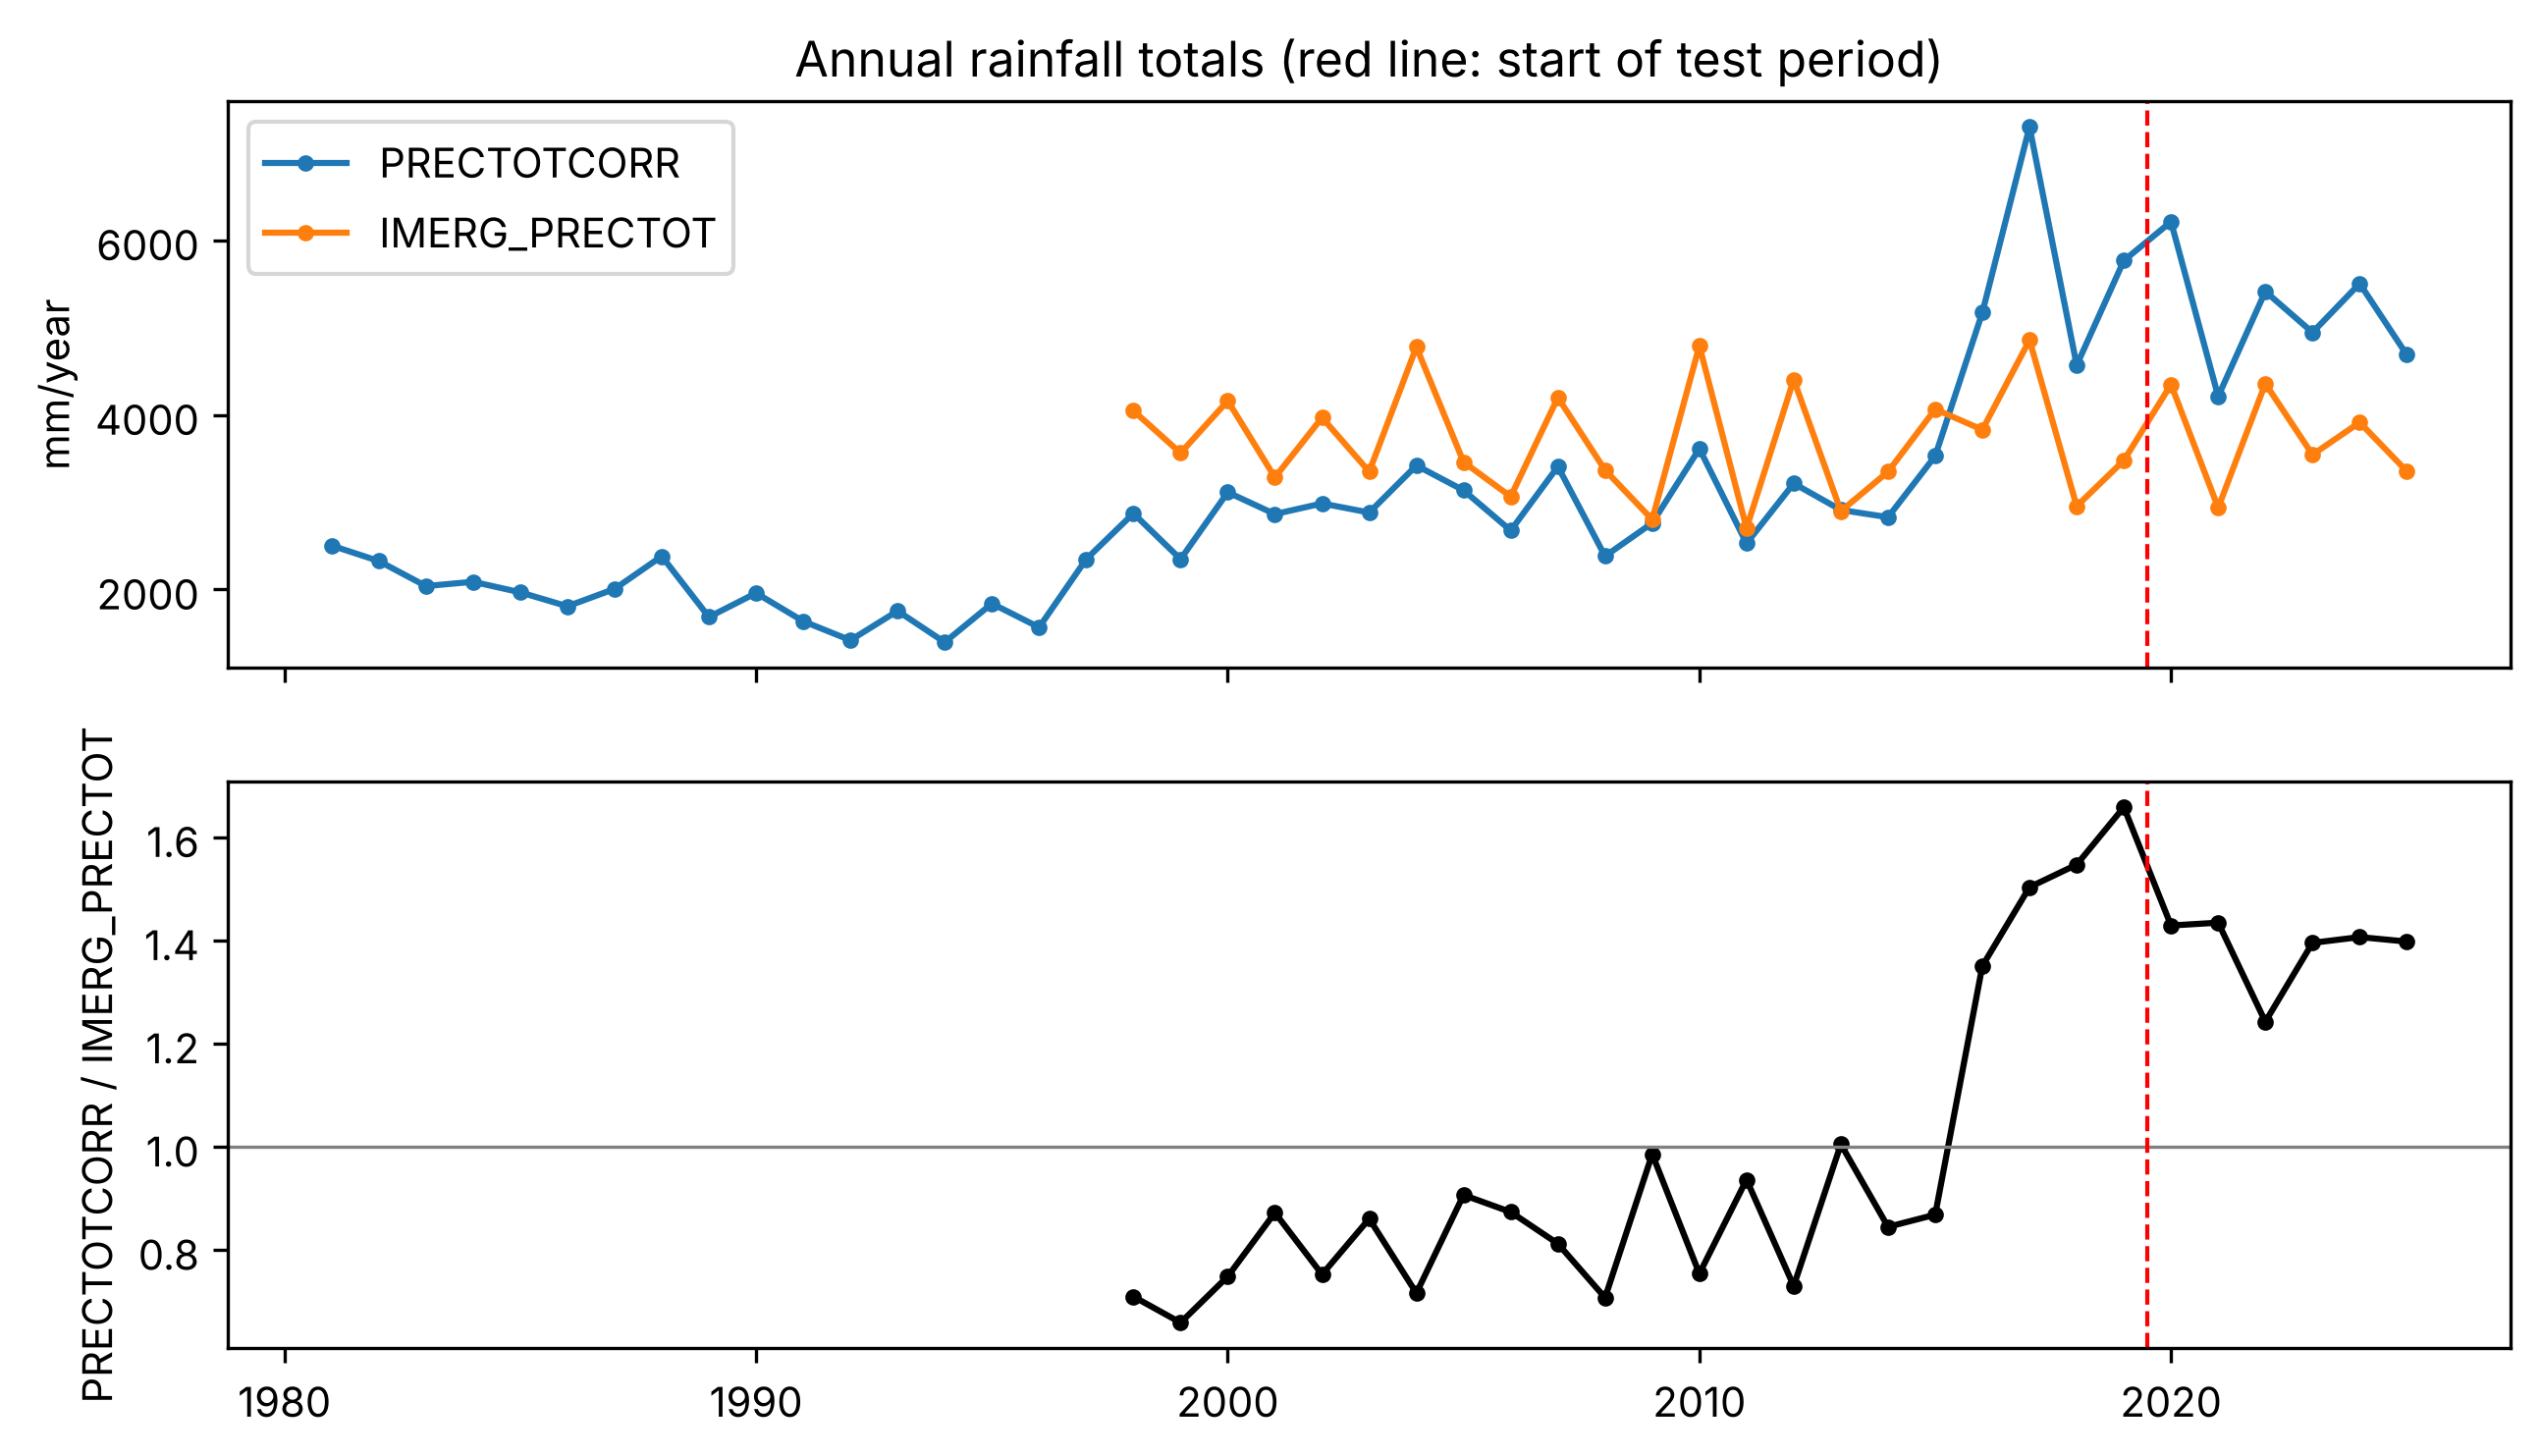
\includegraphics[width=1\textwidth,height=\textheight]{figures/01_annual_totals_and_ratio.png}
\caption{Annual precipitation totals at the study grid cell, 1981--2025. Top: MERRA-2 bias-corrected precipitation (PRECTOTCORR, the forecast target) and IMERG satellite precipitation (1998--2025). Bottom: ratio PRECTOTCORR/IMERG. The step changes of PRECTOTCORR around 2000 and 2016 are absent from IMERG; the red dashed line marks the start of the locked test period (2020).}
\end{figure}

% source: figures/01_annual_totals_and_ratio.png

\begin{figure}
\centering
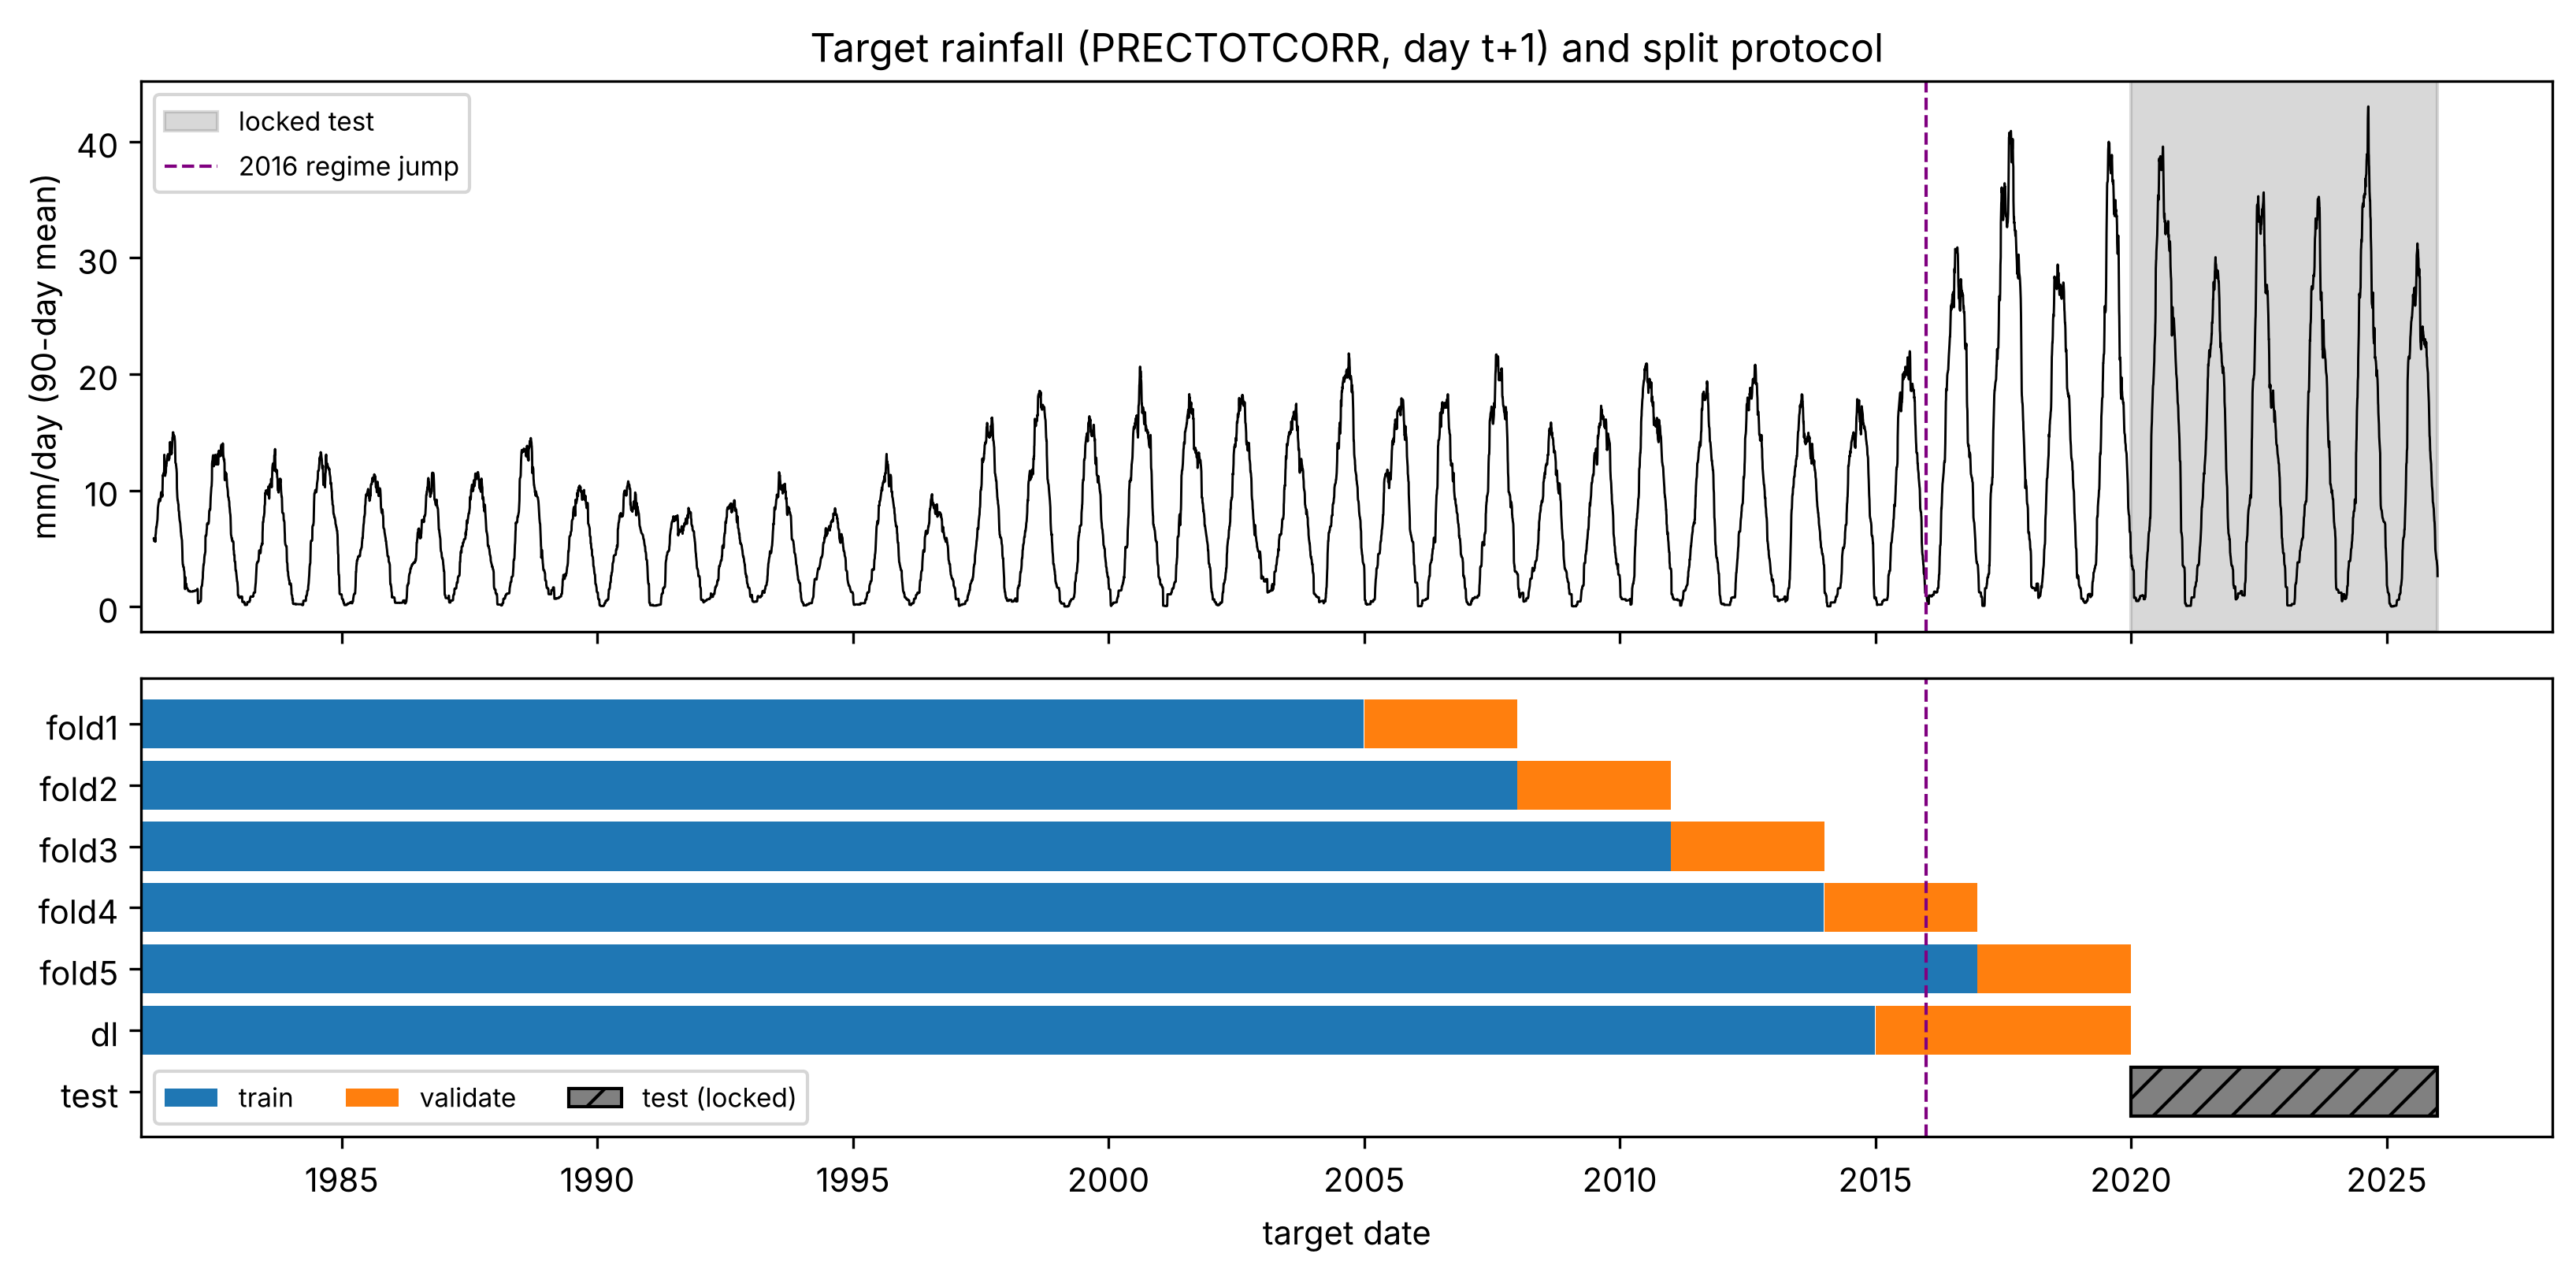
\includegraphics[width=1\textwidth,height=\textheight]{figures/03_split_timeline.png}
\caption{Target series and evaluation design. Top: 90-day running mean of next-day PRECTOTCORR rainfall with the 2016 regime change (dashed) and the locked test period 2020--2025 (shaded). Bottom: the five expanding-window development folds (training in blue, three-year validation blocks in orange), the single split used for the deep models (training to 2014, validation 2015--2019) and the test period, all defined by target date with a one-day purge.}
\end{figure}

% source: figures/03_split_timeline.png

\begin{figure}
\centering
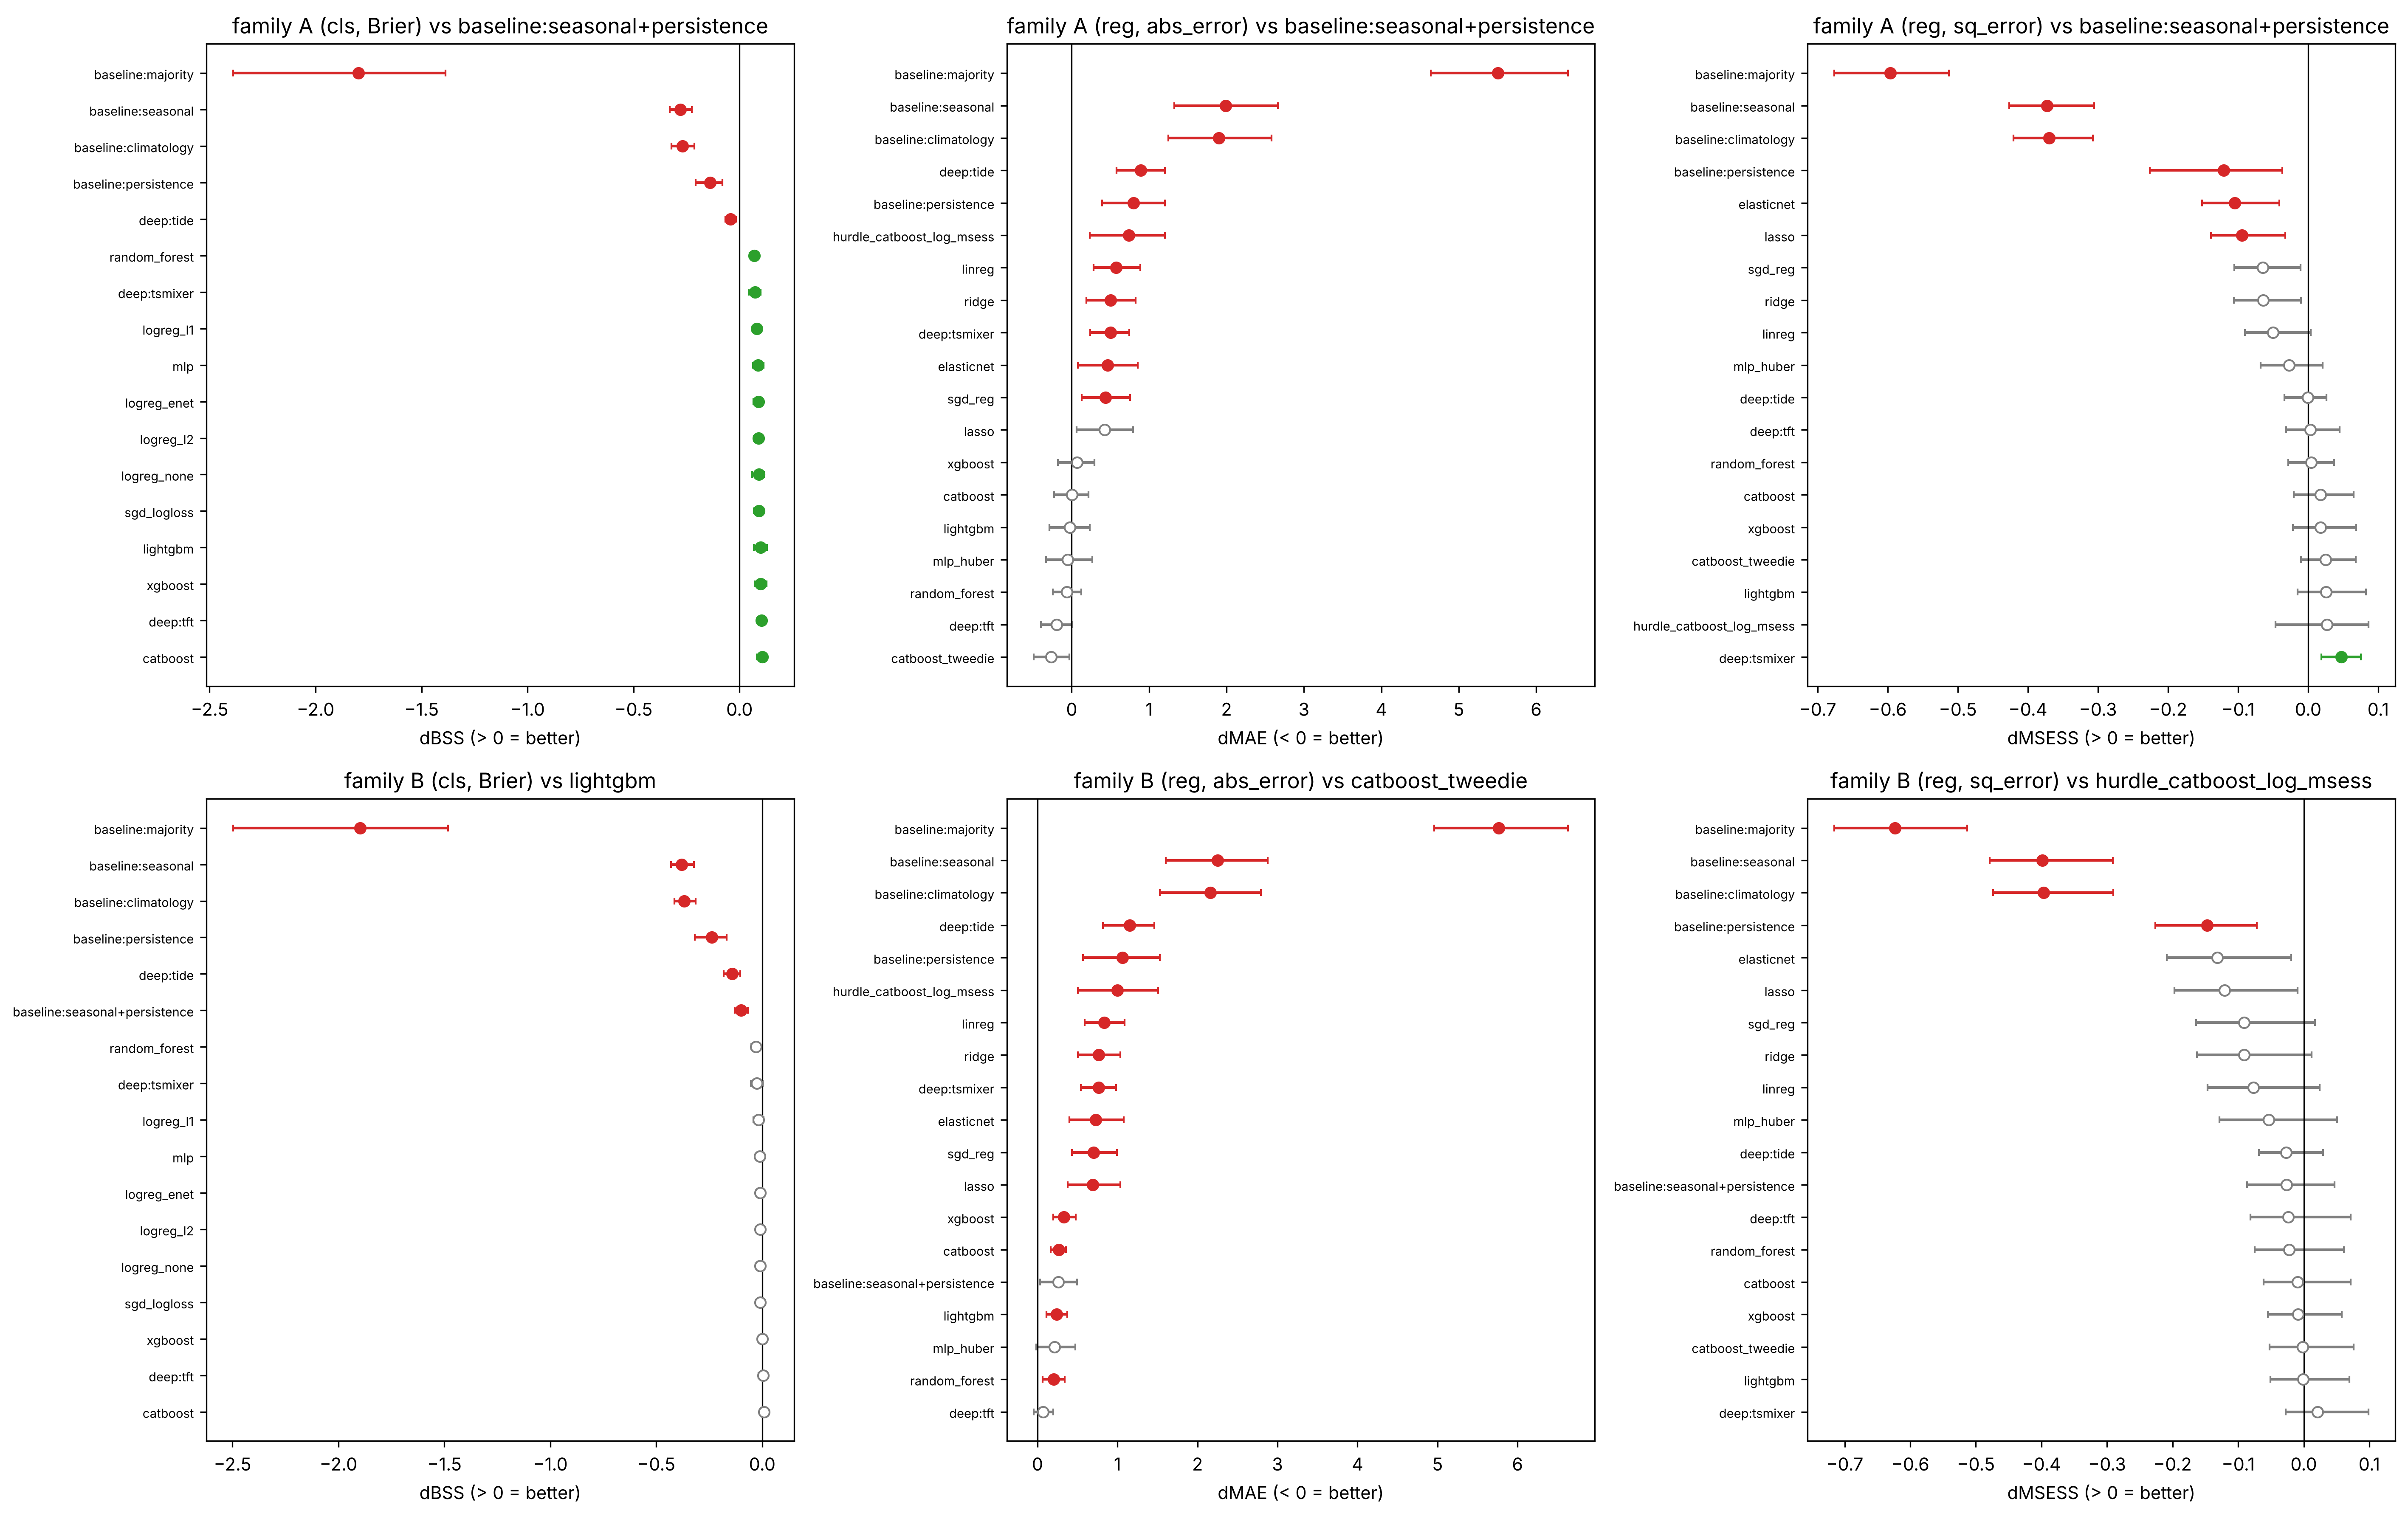
\includegraphics[width=1\textwidth,height=\textheight]{figures/07_test_forest.png}
\caption{Paired test-set effect sizes with 95 \% monthly block-bootstrap confidence intervals. Top row: family A, every model versus seasonal + persistence; bottom row: family B, every model versus the pre-declared headline reference (LightGBM for the Brier score, CatBoost Tweedie for absolute error, the hurdle model for squared error). Columns: $\Delta$BSS (\textgreater{} 0 better), $\Delta$MAE in mm (\textless{} 0 better) and $\Delta$MSESS (\textgreater{} 0 better). Filled markers: significant after Holm correction of Diebold--Mariano tests (green better, red worse); open markers: not significant.}
\end{figure}

% source: figures/07_test_forest.png

\begin{figure}
\centering
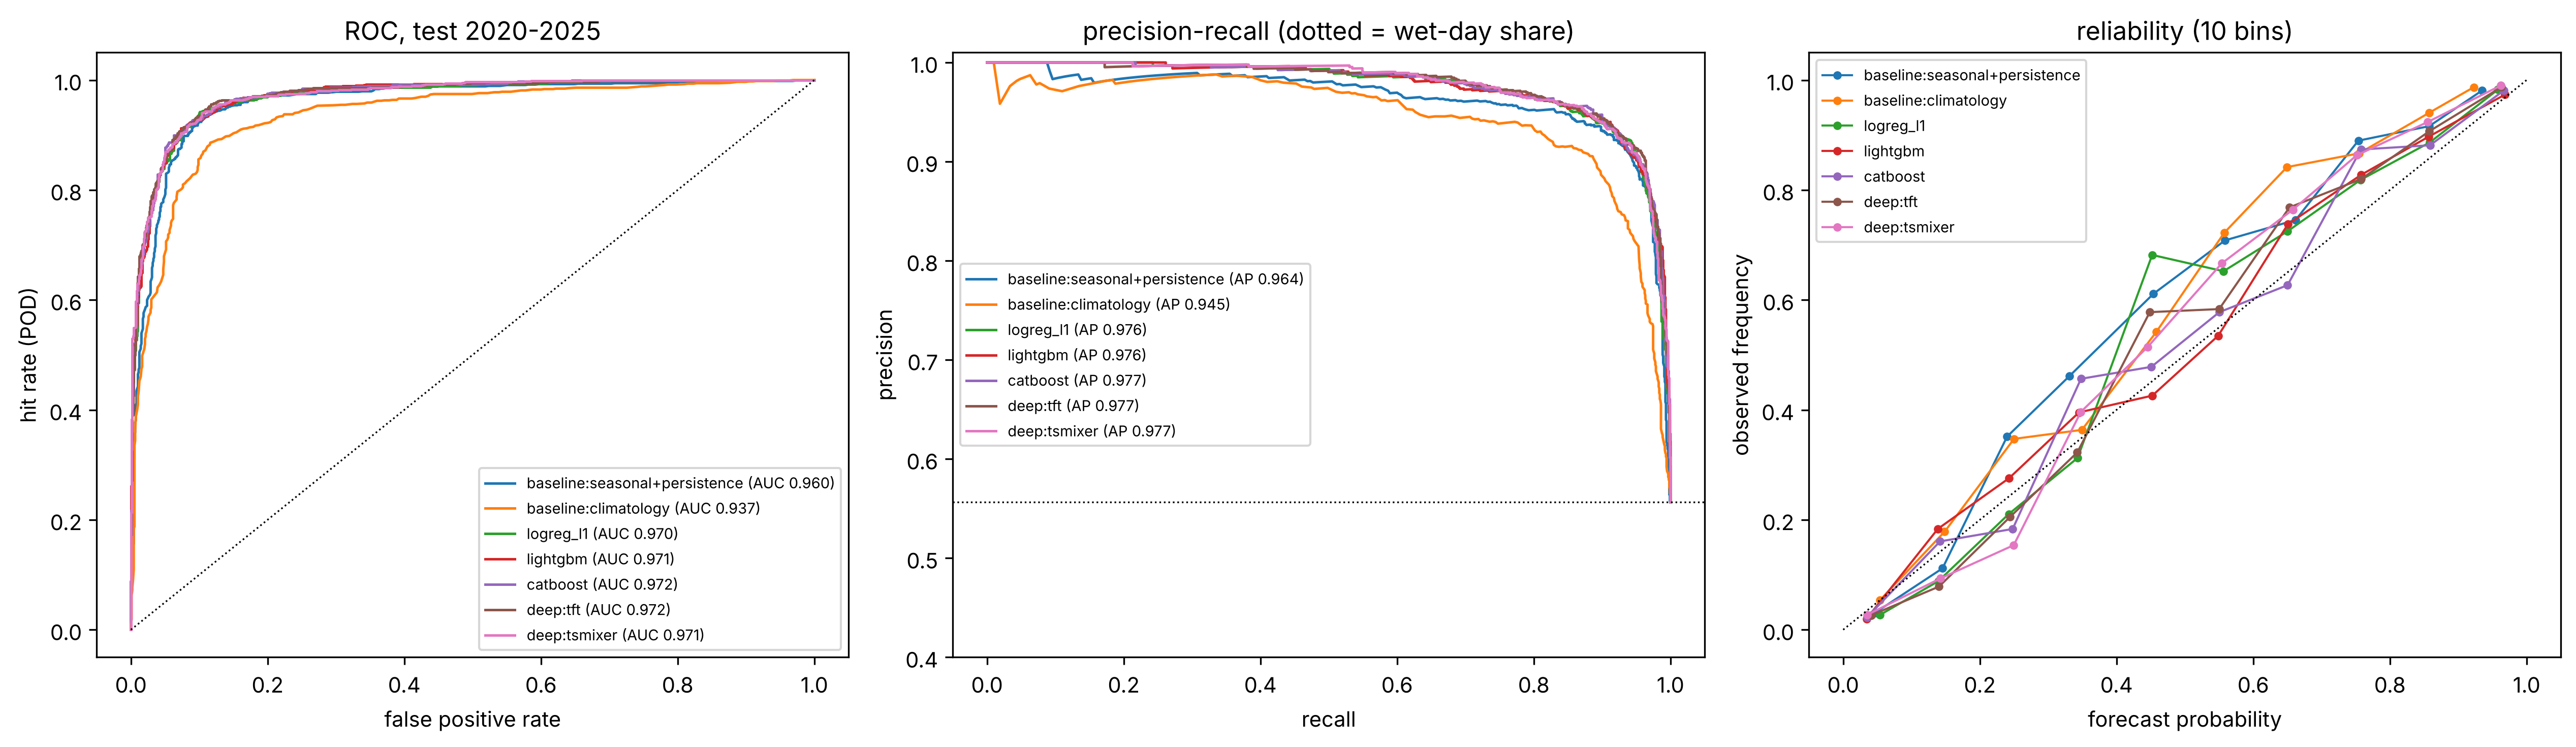
\includegraphics[width=1\textwidth,height=\textheight]{figures/07_test_roc_pr_reliability.png}
\caption{Test-set (2020--2025) verification of rain-occurrence probabilities ($\ge$ 1 mm) for the seed-mean forecasts of the main classifiers and two baselines: receiver operating characteristic curves with ROC-AUC (left), precision--recall curves with average precision, the dotted line marking the wet-day share (centre), and reliability diagrams with 10 equal-width probability bins (right).}
\end{figure}

% source: figures/07_test_roc_pr_reliability.png

\begin{figure}
\centering
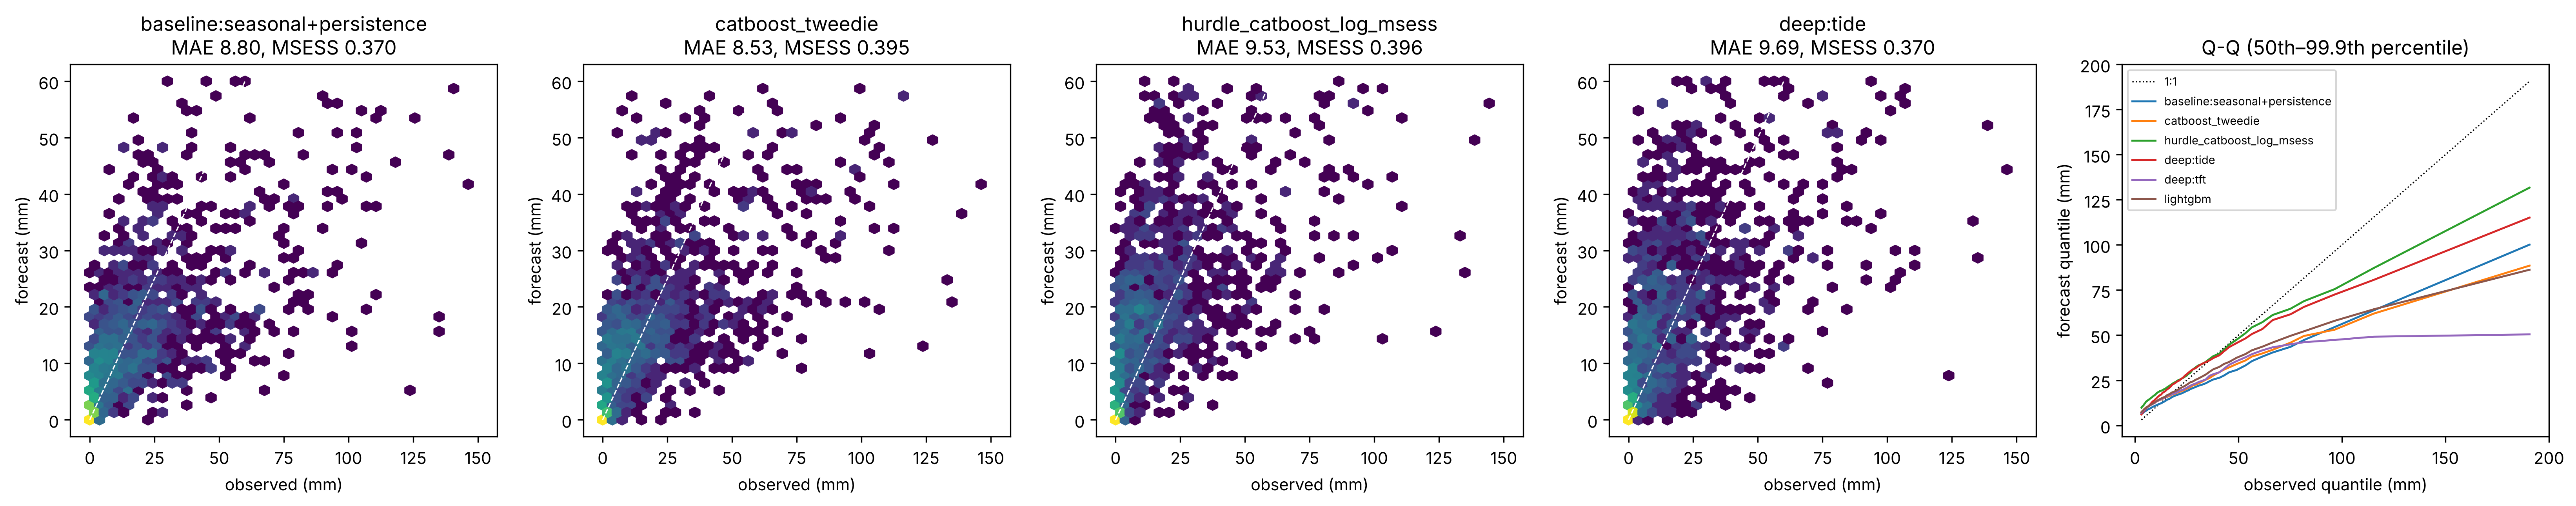
\includegraphics[width=1\textwidth,height=\textheight]{figures/07_test_pred_vs_obs.png}
\caption{Test-set rainfall amount forecasts versus observations for seasonal + persistence, CatBoost Tweedie, the hurdle model and TiDE (hexagonal density plots with MAE and MSESS in the panel titles), and quantile--quantile comparison of forecast and observed distributions from the 50th to the 99.9th percentile (right), showing that all models compress the upper tail.}
\end{figure}

% source: figures/07_test_pred_vs_obs.png

\begin{figure}
\centering
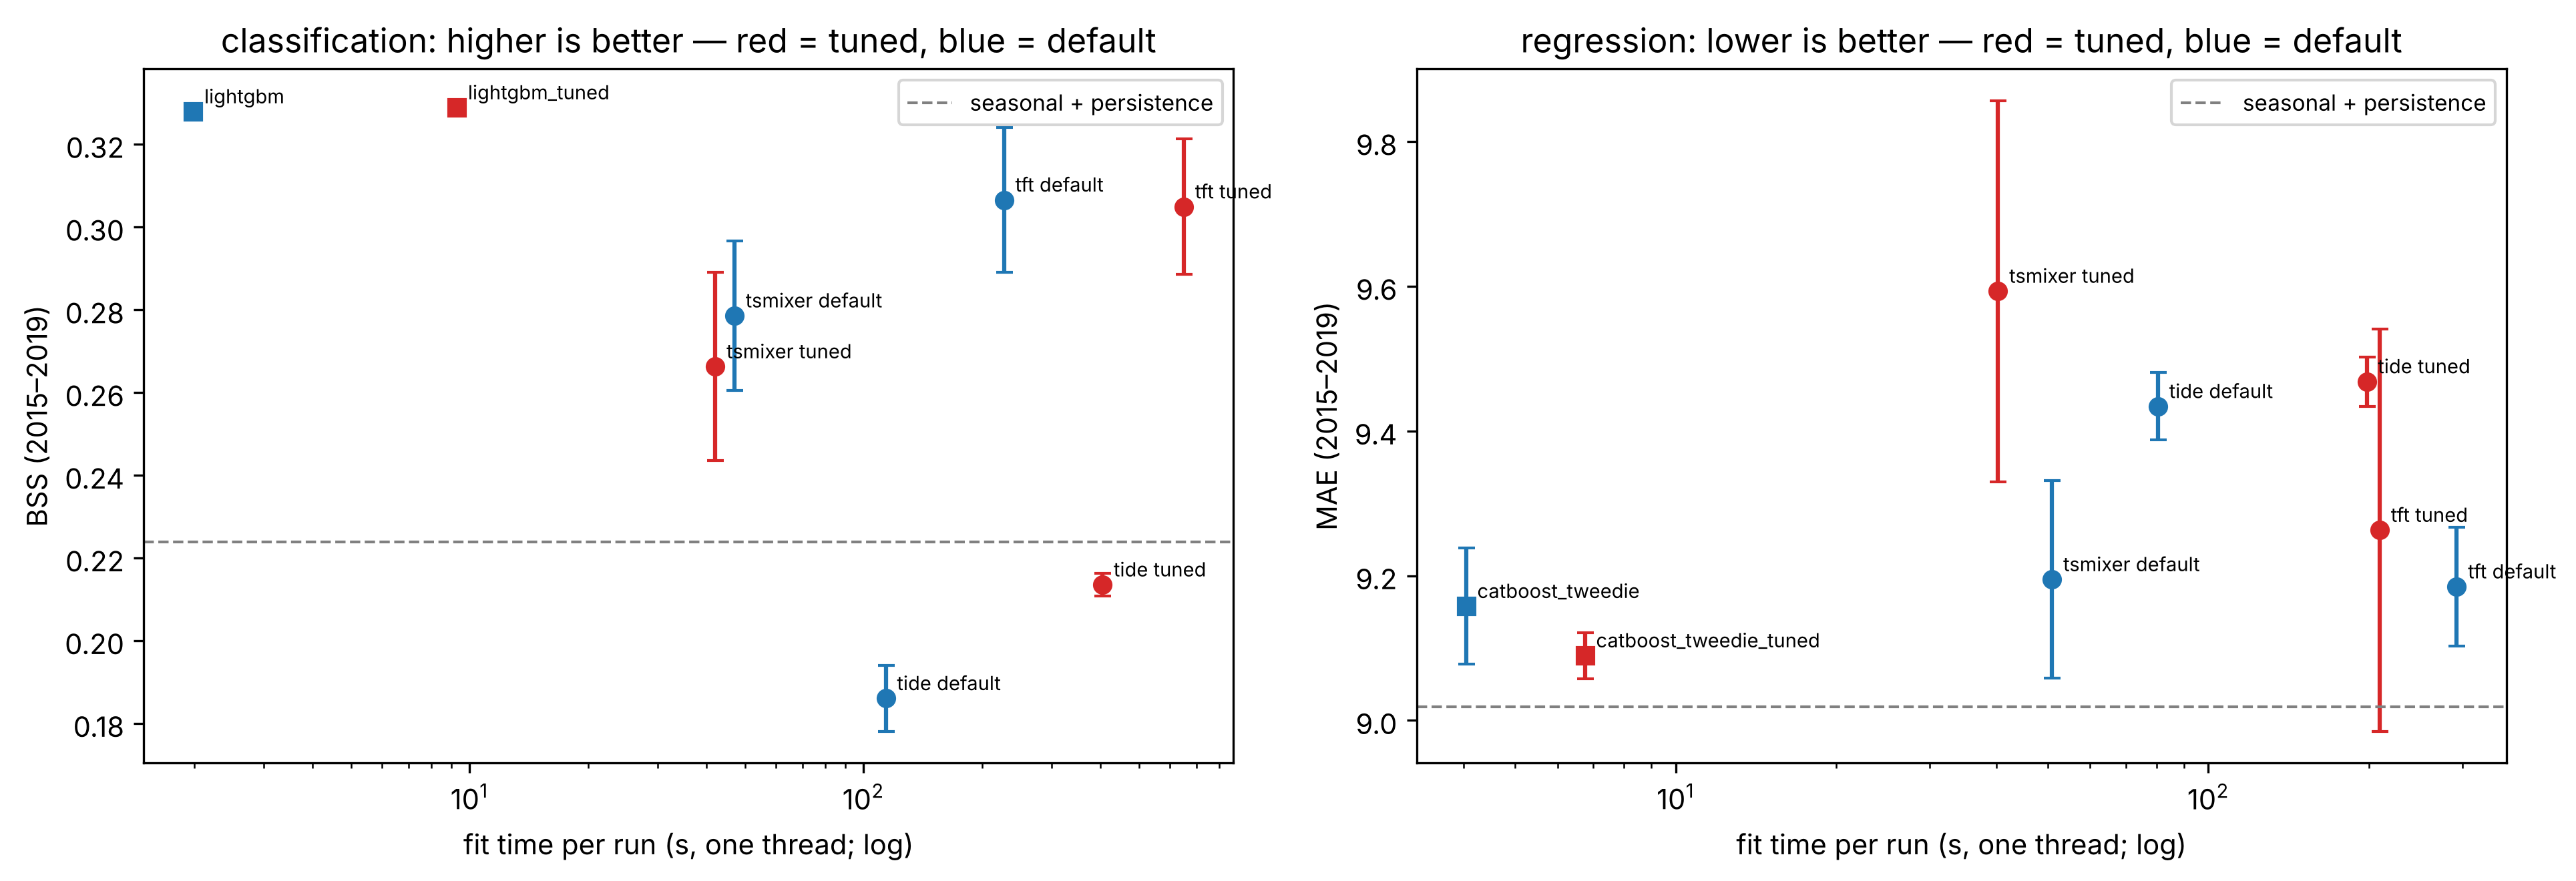
\includegraphics[width=1\textwidth,height=\textheight]{figures/06_deep_cost_vs_skill.png}
\caption{Skill versus single-thread training time per fit on the deep-learning split (validation 2015--2019) for default (blue) and tuned (red) configurations. Left: classification BSS (higher is better); right: regression MAE in mm (lower is better). Squares: gradient-boosted trees; circles: deep sequence models; error bars: $\pm$ one standard deviation over five seeds; dashed line: seasonal + persistence. Time axis logarithmic.}
\end{figure}

% source: figures/06_deep_cost_vs_skill.png

\begin{figure}
\centering
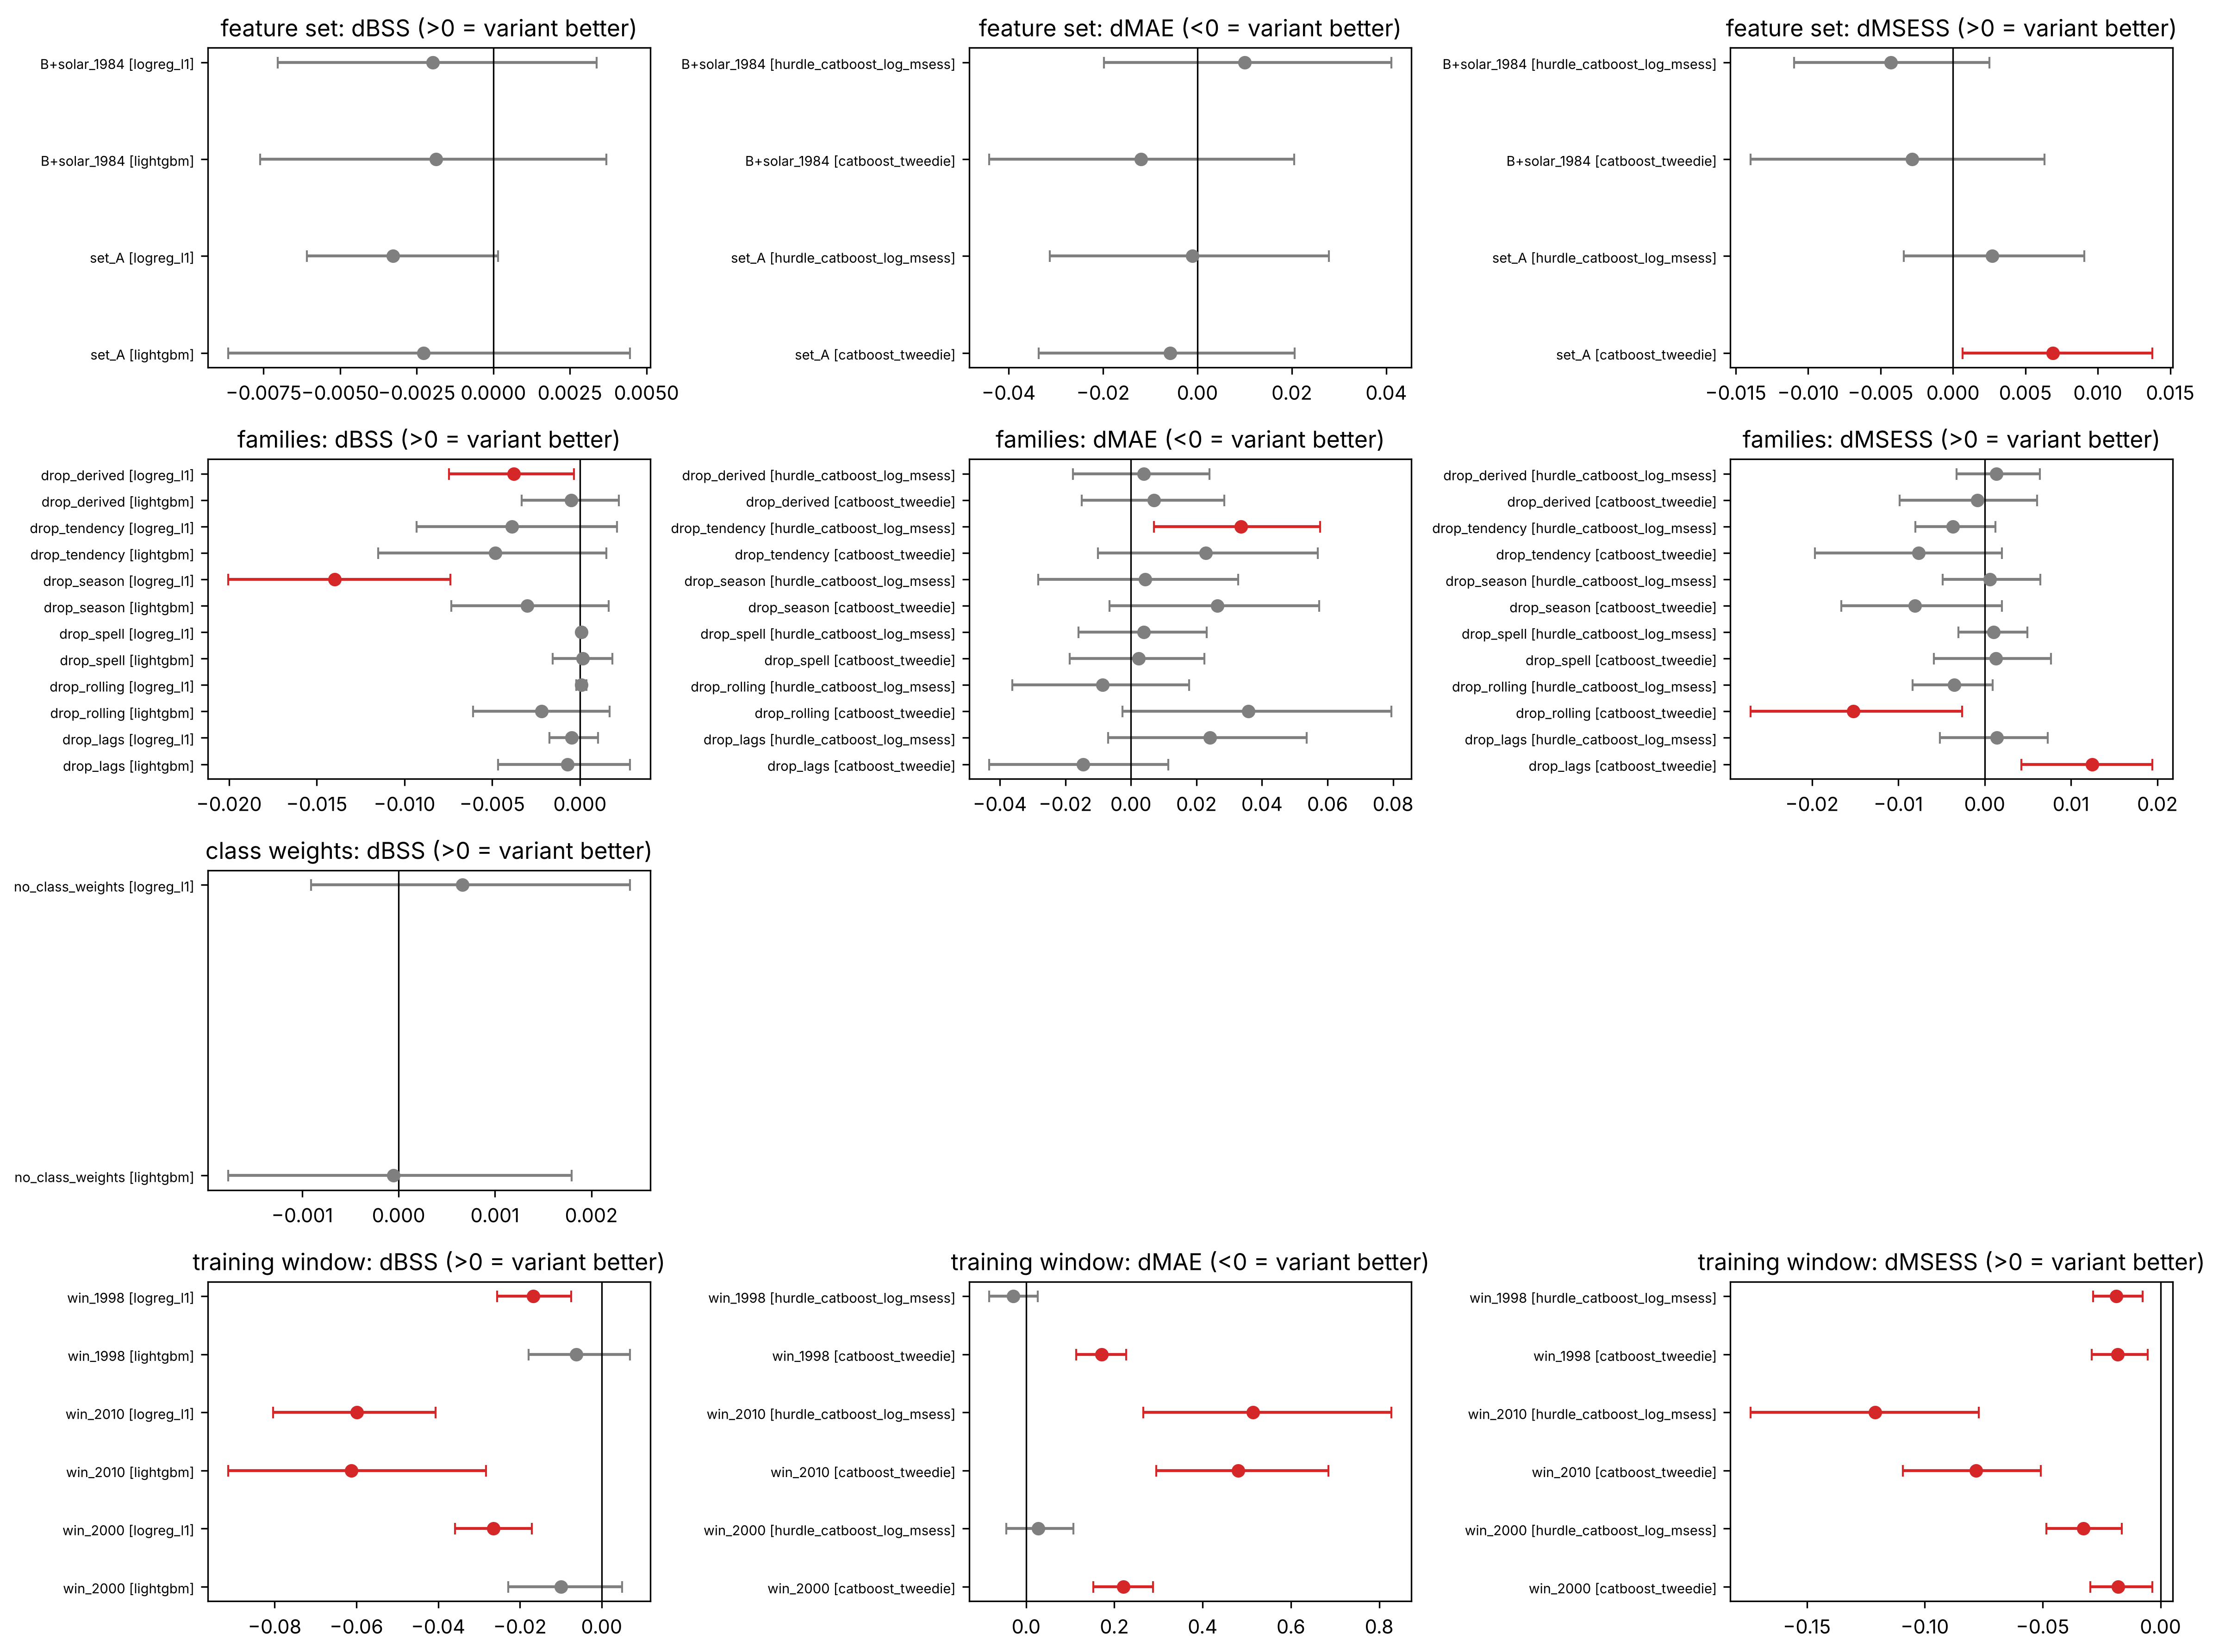
\includegraphics[width=1\textwidth,height=\textheight]{figures/06_ablation_forest_classical.png}
\caption{Ablation effects on the development folds for the classical models (LightGBM, L1-logistic regression, CatBoost Tweedie and the hurdle model): feature sets, removal of feature families, class weights and training windows. Points are differences from the full configuration with uncorrected 95 \% monthly block-bootstrap intervals; red intervals exclude zero. Signs: $\Delta$BSS and $\Delta$MSESS \textgreater{} 0 and $\Delta$MAE \textless{} 0 mean that the variant is better.}
\end{figure}

% source: figures/06_ablation_forest_classical.png

\begin{figure}
\centering
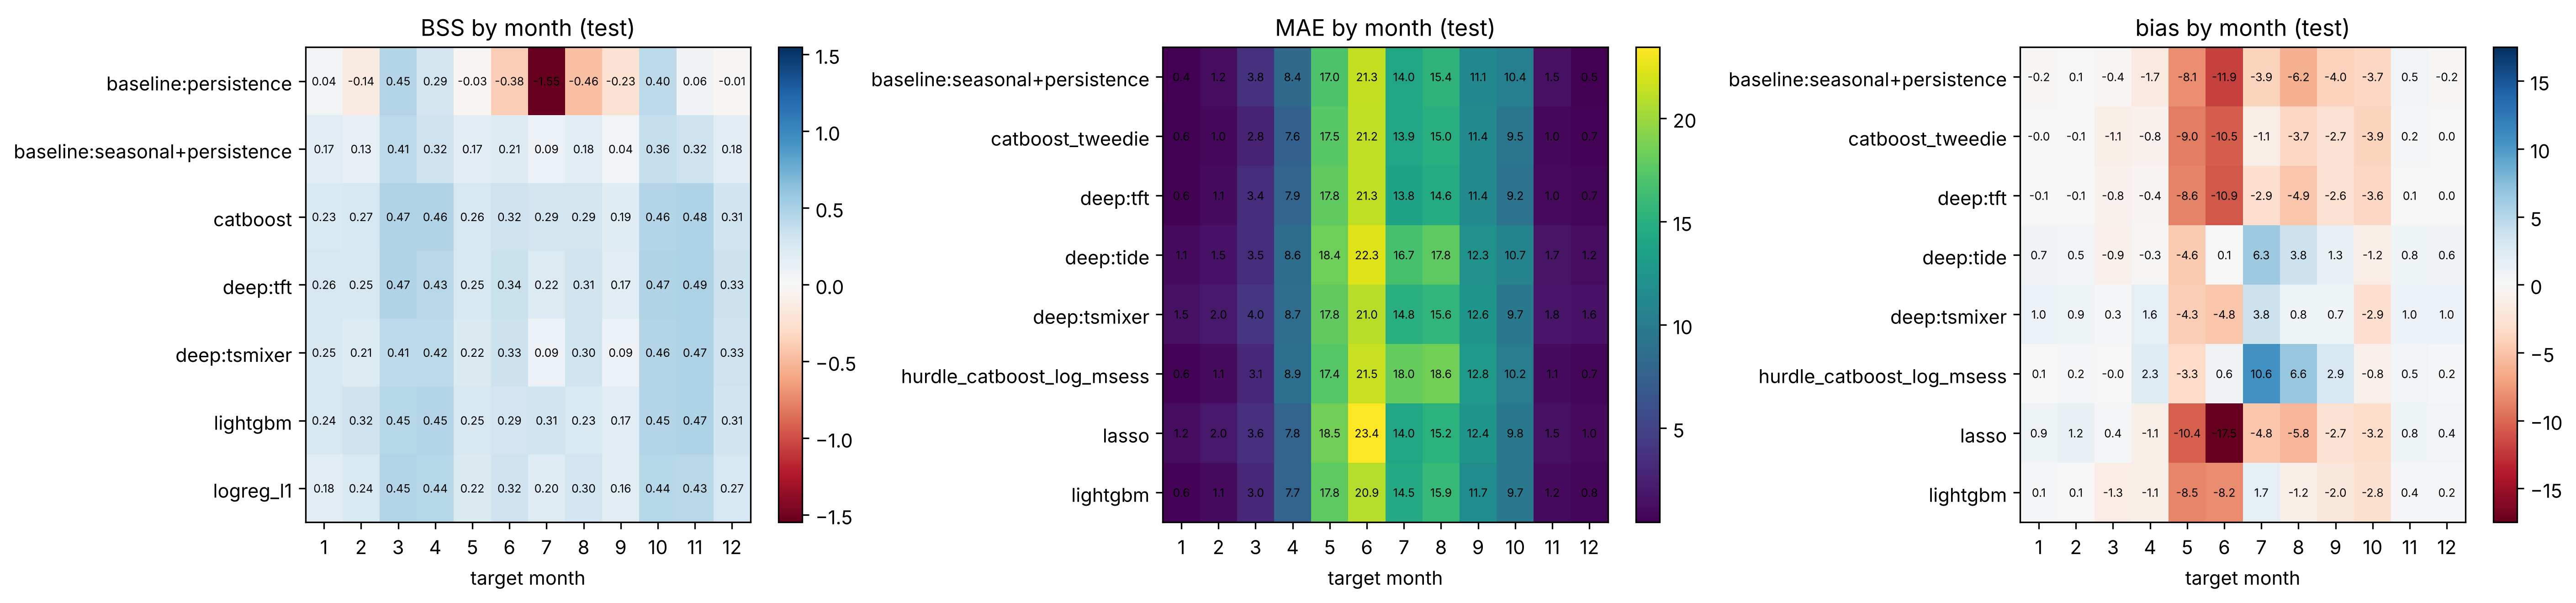
\includegraphics[width=1\textwidth,height=\textheight]{figures/08_errors_by_month.png}
\caption{Test-set performance by target month: BSS of the classifiers (left), MAE in mm (centre) and bias in mm/day (right) of the amount models. Skill is highest in the transition months (March--April, October--November) and lowest in the core monsoon, where errors and negative biases are largest.}
\end{figure}

% source: figures/08_errors_by_month.png

\begin{figure}
\centering
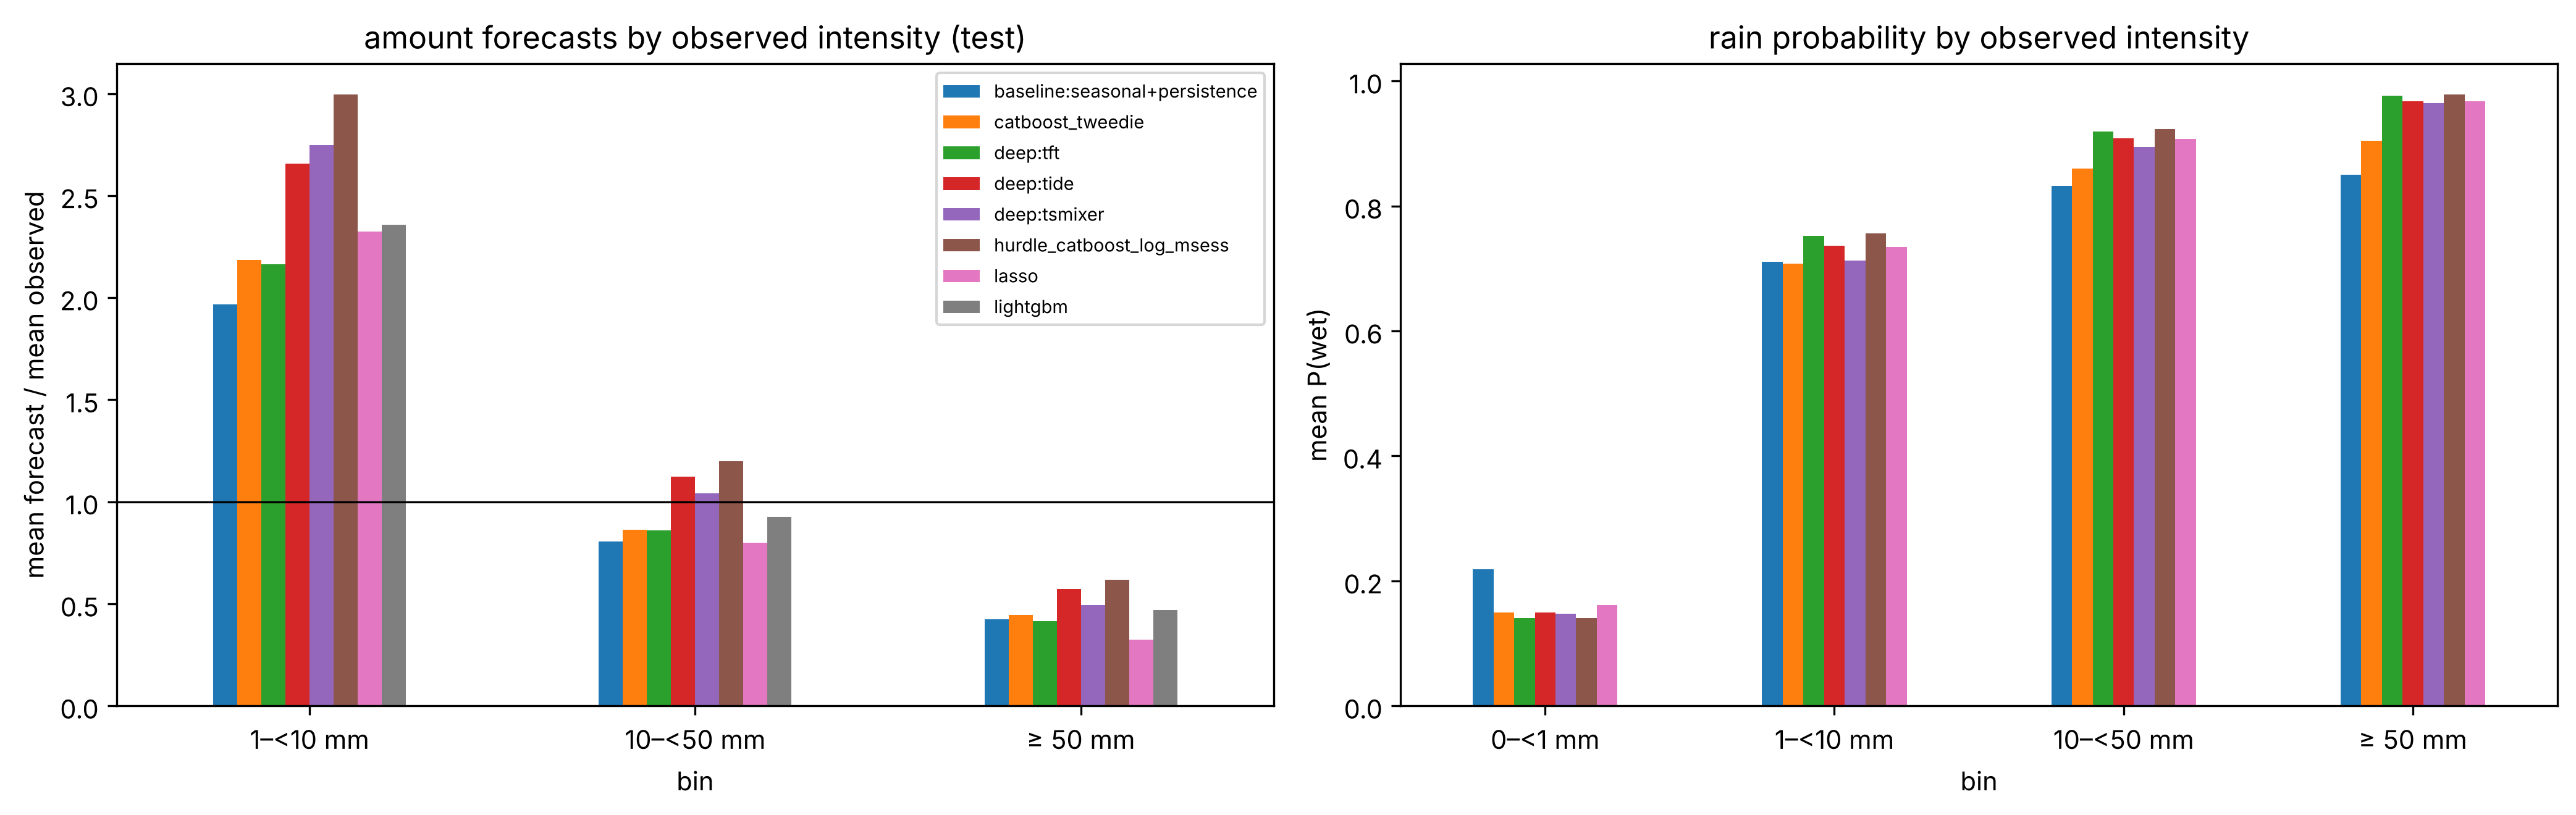
\includegraphics[width=1\textwidth,height=\textheight]{figures/08_errors_by_intensity.png}
\caption{Test-set forecasts stratified by observed rainfall intensity. Left: ratio of mean forecast to mean observed amount for days of 1--\textless10 mm, 10--\textless50 mm and $\ge$ 50 mm (horizontal line: unbiased); light rain is over-forecast and heavy rain is damped by all models. Right: mean forecast probability of rain for each intensity class.}
\end{figure}

% source: figures/08_errors_by_intensity.png

\begin{figure}
\centering
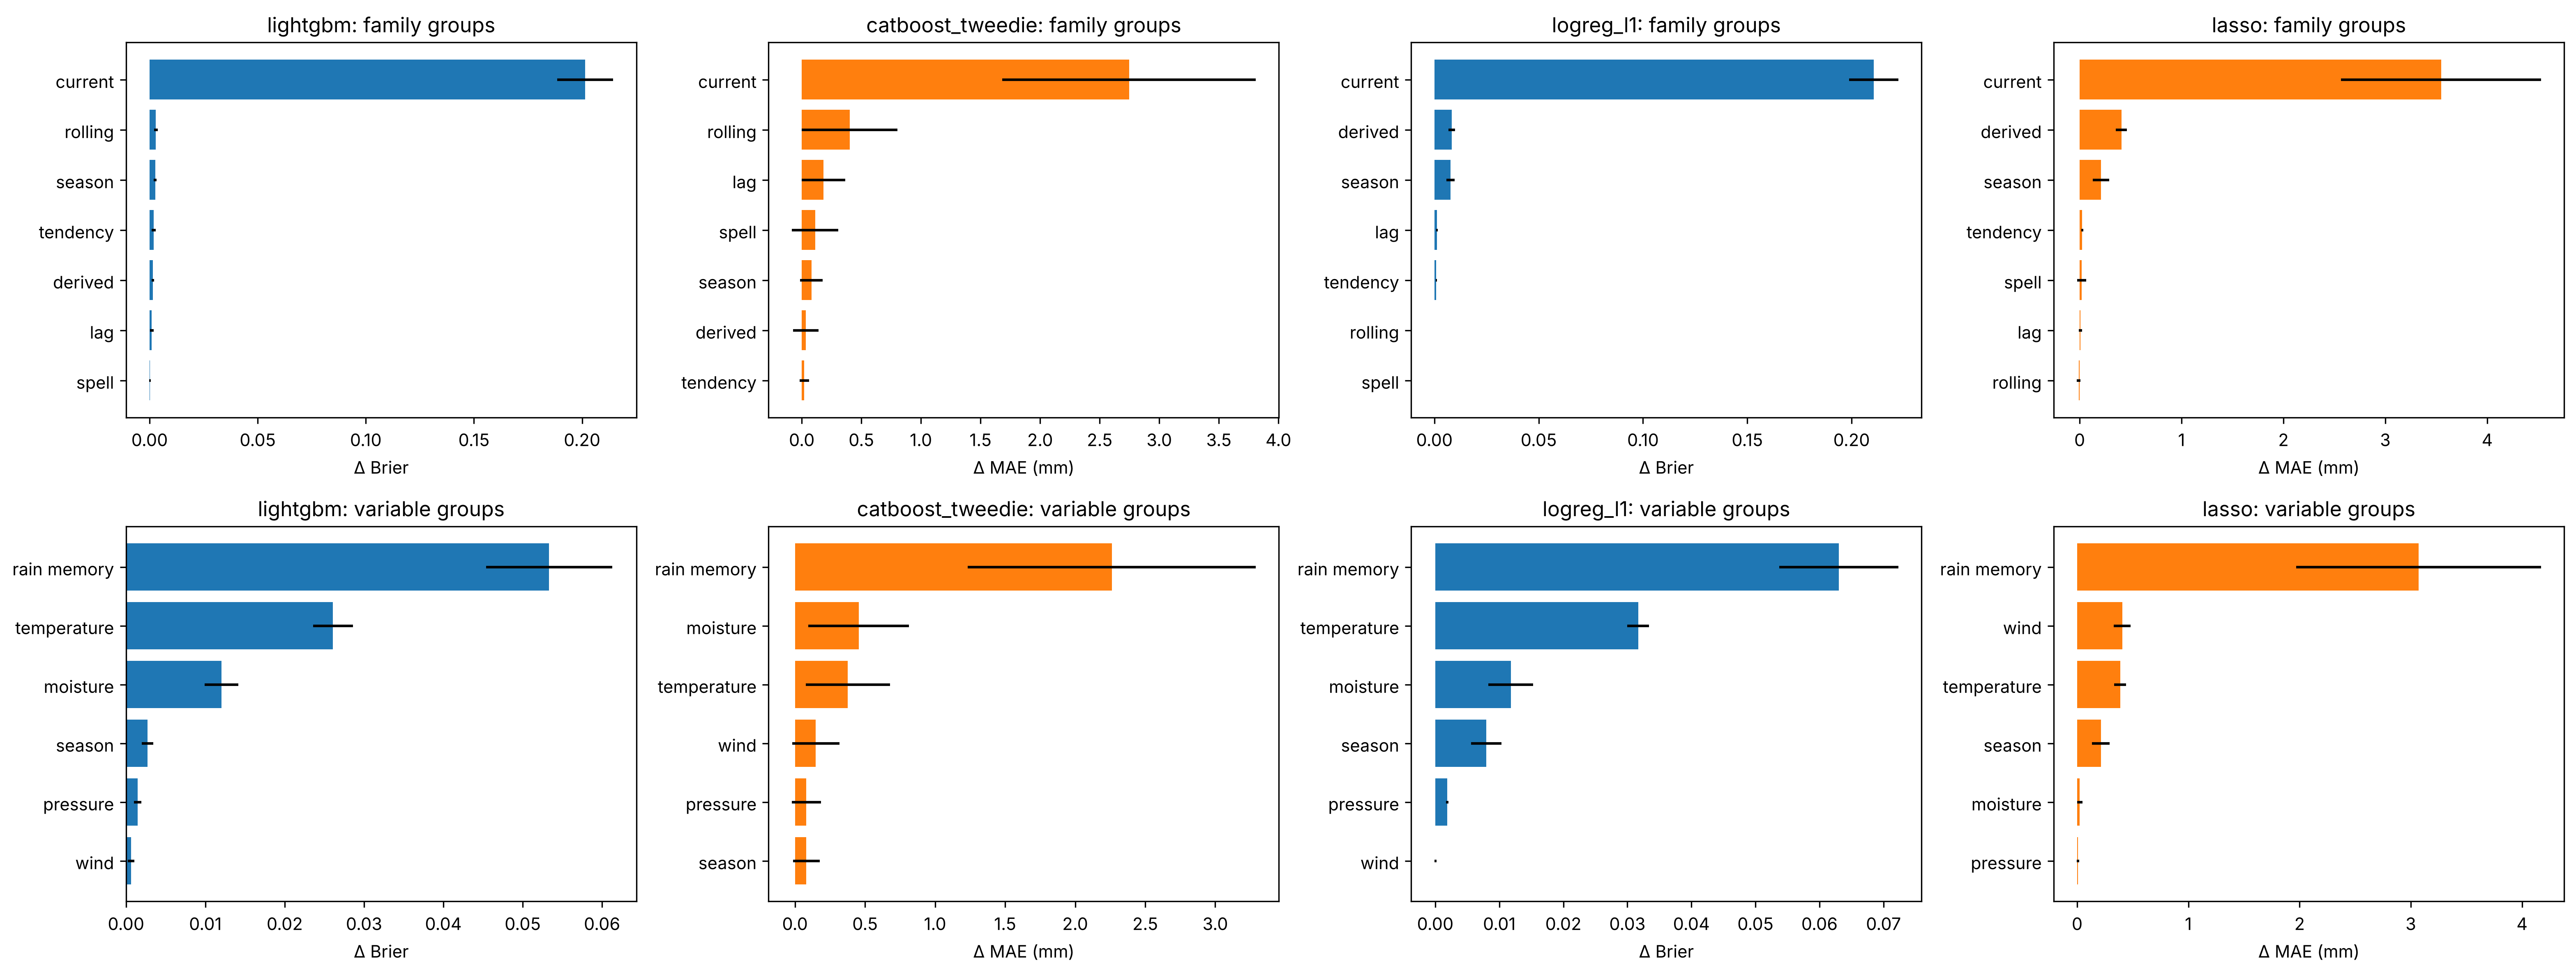
\includegraphics[width=1\textwidth,height=\textheight]{figures/08_permutation_importance_groups.png}
\caption{Grouped permutation importance on the development validation folds (2005--2019) for LightGBM, CatBoost Tweedie, L1-logistic regression and lasso. Top: groups by feature-engineering family; bottom: groups by physical variable. Bars show the increase in Brier score or MAE when all columns of a group are permuted jointly; error bars show the variability across folds and repeats.}
\end{figure}

% source: figures/08_permutation_importance_groups.png

Supplementary figures (all in \texttt{reports/figures/}, 300 dpi):

\begin{itemize}
\tightlist
\item
  \texttt{00\_missing\_by\_year.png}
\item
  \texttt{00\_wd2m\_break.png}
\item
  \texttt{01\_acf\_pacf.png}
\item
  \texttt{01\_monthly\_climatology.png}
\item
  \texttt{03\_baseline\_regime\_check.png}
\item
  \texttt{05\_tft\_quantiles.png}
\item
  \texttt{05\_tft\_explainability.png}
\item
  \texttt{06\_ablation\_imerg.png}
\item
  \texttt{06\_ablation\_threshold.png}
\item
  \texttt{06\_ablation\_window\_by\_fold.png}
\item
  \texttt{06\_ablation\_lookback.png}
\item
  \texttt{06\_default\_vs\_tuned\_paired.png}
\item
  \texttt{07\_test\_by\_season.png}
\item
  \texttt{07\_test\_timeseries.png}
\item
  \texttt{08\_errors\_by\_year.png}
\item
  \texttt{08\_transitions.png}
\item
  \texttt{08\_calibration\_by\_season.png}
\item
  \texttt{08\_shap\_beeswarm.png}
\item
  \texttt{08\_ale\_pdp.png}
\item
  \texttt{08\_linear\_coefficients.png}
\end{itemize}

\textbf{Tables.} Table 1: test-set classification scores. Table 2: paired classification comparisons with Holm-adjusted DM tests. Table 3: test-set regression scores. Table 4: paired regression comparisons with Holm-adjusted DM tests. All tables are generated by \texttt{notebooks/09\_paper\_tables.ipynb} from the CSV files in \texttt{reports/tables/}.

  \bibliography{references}

\end{document}
